\documentclass[brazil,ruledheader]{abntifes}
%\documentclass[brazil,twoside,ruledheader]{abntifes}
\usepackage[T1]{fontenc} 
%\usepackage[latin1]{inputenc}
\usepackage[utf8]{inputenc}
\usepackage[brazil]{babel}
\usepackage[]{algorithm2e}
\usepackage{pslatex}
\usepackage{url}
\usepackage{fancyhdr}
\usepackage{graphicx}
\usepackage{amsmath, amsthm, amssymb}
\usepackage{exercise}
\usepackage{makeidx}
\usepackage{setspace}
\usepackage{multicol}    
\usepackage{upquote}
\usepackage{graphicx}
\usepackage{float}
\usepackage{epigraph}

\usepackage{listings}

\lstset{numbers=left, stepnumber=5, firstnumber=1, numberstyle=\tiny, extendedchars=true, breaklines=true, frame=tb, basicstyle=\footnotesize, stringstyle=\ttfamily, showstringspaces=false }

%\makenomenclature

% Para listar programas em C# 
\lstdefinelanguage{cs}
{morekeywords={abstract,event,new,struct,as,explicit,null,switch
		base,extern,object,this,bool,false,operator,throw,
		break,finally,out,true,byte,fixed,override,try,
		case,float,params,typeof,catch,for,private,uint,
		char,foreach,protected,ulong,checked,goto,public,unchecked,
		class,if,readonly,unsafe,const,implicit,ref,ushort,
		continue,in,return,using,decimal,int,sbyte,virtual,
		default,interface,sealed,volatile,delegate,internal,short,void,
		do,is,sizeof,while,double,lock,stackalloc,
		else,long,static,enum,namespace,string, },
	sensitive=false,
	morecomment=[l]{//},
	morecomment=[s]{/*}{*/},
	morestring=[b]",
}

\newcommand{\AUTOR}{João Pedro Souza Homem}
\newcommand{\SEGUNDOAUTOR}{}
\newcommand{\ORIENTADOR}{Marlan Kulberg}
\newcommand{\COORIENTADOR}{}
\newcommand{\TITULO}{Aplicação tempo-real com NodeJS - Chat por localização geográfica}
\newcommand{\CURSO}{Tecnólogo em Tecnologia da Informação e Comunicação}
\newcommand{\GRAU}{Tecnólogo em Tecnologia da Informação e Comunicação}
% \newcommand{\GRAU}{Tecnólogo em Análise e Desenvolvimento de Sistemas}
\newcommand{\INSTITUICAO}{Faculdade de Educação Tecnológica do Estado do Rio de Janeiro Faeterj/Petrópolis}
\newcommand{\ANO}{Dezembro, 2016}
\newcommand{\DATA}{12 de Dezembro de 2016}
\newcommand{\LOCAL}{Petrópolis - RJ}
\newcommand{\epigrafe}{\vspace{1cm}{\raggedright\par\sffamily\slshape\par}}
\begin{document}
	
	\autor{\AUTOR}
	\titulo{\TITULO}
	\orientador{\ORIENTADOR}
	\coorientador{\COORIENTADOR}
	
	\comentario{Trabalho de Conclusão de Curso apresentado à Coordenadoria do Curso de \CURSO\
		da \INSTITUICAO , como requisito parcial para obtenção do título de \GRAU .}
	
	\instituicao{\INSTITUICAO}
	\curso{\CURSO}
	\governo{Governo do Estado do Rio de Janeiro}
	\secretaria{Secretaria de Estado de Ciência e Tecnologia}
	\fundacao{Fundação de Apoio à Escola Técnica}
	\cpti{Centro de Educação Profissional em Tecnologia da Informação}
	\local{\LOCAL}
	\data{\ANO}
	
	\capa
	
	\folhaderosto
	
	% Ficha Catalográfica
	%\begin{figure}
	%\includegraphics[width=11cm]{FichaCatalografica.pdf}
	%\end{figure}
	
	% Folha de Aprovação
	\newpage
	\vfill 
	\null
	\begin{center}
		{\Huge {\bfseries\itshape Folha de Aprovação}}\\[3cm]
		\begin{espacoduplo}
			Trabalho de Conclusão de Curso sob o título \textit{``\TITULO''},
			defendida por \AUTOR\ e aprovada em \DATA, em \LOCAL, pela banca examinadora constituída pelos
			professores: \setlength{\ABNTsignthickness}{0.4pt}
		\end{espacoduplo}
		\setlength{\ABNTsignthickness}{0.4pt}
		
		% ou inserir a página assinada e escaneada aqui
		%\begin{figure}
		%\includegraphics[]{Fo	lhaAprovacao.pdf}
		%\end{figure}
		
		
		\assinatura{Prof. \ORIENTADOR\\ Orientador} 
		\assinatura{Prof. Banca Interna \\ \INSTITUICAO} 
		\assinatura{Prof. Banca Interna \\ \INSTITUICAO} 
		%\assinatura{Prof. Banca Externa \\ Instituto do membro externo}
		
	\end{center}
	
	
	% Folha do Termo de Compromisso
	\newpage
	
	\vfill 
	\null
	\begin{center}
		{\Huge {\bfseries\itshape Declaração de Autor}}\\[3cm]
		\begin{espacoduplo}
			Declaro, para fins de pesquisa acadêmica, didática e técnico-científica, que o presente Trabalho de Conclusão
			de Curso pode ser parcial ou totalmente utilizado desde que se faça referência à fonte e aos autores.
		\end{espacoduplo}
		\setlength{\ABNTsignthickness}{0.4pt}
		\assinatura{\AUTOR}
		Petrópolis, em \DATA
	\end{center}
	
	\chapter*{Agradecimentos}
	Agradeço a todos que de forma direta ou indireta contribuíram para a elaboração deste trabalho através do investimento em minha capacitação, compartilhamento de conhecimento, disponibilização de ferramentas e componentes para desenvolvimento de \textit{softwares}, entre outros não menos importantes.
	
	Dentre todos os relacionados a este agradecimento, gostaria especialmente de agradecer a toda comunidade \textit{open-source}, da qual pude usufruir de diversos recursos que viabilizaram a implementação da aplicação abordada neste documento. A iniciativa \textit{open-source} abre muitos caminhos para a inovação e inclusão na área de desenvolvimento de \textit{softwares} e deve ser incentivada e reconhecida, atribuindo-se os devidos méritos a cada um que adere a iniciativa em seus projetos.
	\vfill 
	\null
	
	\begin{center}
		{\Huge {\bfseries\itshape Epígrafe}}\\[3cm]
		\vspace{15cm}
	\end{center}
	
	\begin{espacoduplo}
	\end{espacoduplo}
	
	% Epigrafe
	\epigraph{"Faça-se simples com ideias complicadas"}{(JoPaseho)}
	
	% Resumo
	\begin{resumo}
		A evolução da tecnologia vem trazendo para as nossas vida diversas inovações que estão mudando a forma de lidar com inúmeras situações. Alcançamos novos patamares em como tratamos os negócios, relações pessoais, a busca por novos conhecimentos, entre outras coisas. Tudo isso nos levou a buscar entender um tipo de aplicação que tem se tornado cada vez mais presente nas ferramentas que utilizamos.
		
		As aplicações tempo-real são o propósito da realização deste trabalho. Primeiramente, buscamos no mercado algumas referências de aplicações para embasar o desenvolvimento de uma aplicação de \textit{chat} por localização geográfica. Encontramos em nossas referências diversos aspectos que foram considerados para a escolha de como e 
		quais tecnologias usar para construir as funcionalidades.
		
		Tendo como base todas as possibilidades que tínhamos para implementação, delimitamos o problema em construir uma ferramenta com tecnologias modernas e utilizadas no mercado por aplicação com fins semelhantes ao nosso, e que demonstrasse o funcionamento elemental da transmissão de dados em tempo real na \textit{web}.
		
		Sendo assim, subdividimos o desenvolvimento em duas partes principais, que são a aplicação servidor e cliente. 
		
		\begin{itemize}
			\item A aplicação servidor desempenhará o papel de receber as informações da aplicação cliente, processá-las, e distribuí-las para os outros clientes através de uma conexão bidirecional, que nos permite implementar uma comunicação tempo-real entre os diversos usuários da aplicação.
		\end{itemize}
		
		\begin{itemize}
			\item  A aplicação cliente, resumidamente pode ser considerada a interface com a qual os usuários interagem com a aplicação. Através dela o usuário poderá encontrar, por de um mapa terrestre, um outro usuário que esteja utilizando a aplicação no mesmo momento, que será identificado como um ponto marcado no local em que os dados de geolocalização coletados pelo servidor informam. Após a localização do usuário, este poderá ser contactado através de uma janela de comunicação por texto.
		\end{itemize}
		
		A arquitetura utilizada foi inspirada em alguns padrões que moldam a infraestrutura da aplicação para privilegiar ações de escalabilidade, portanto apresentamos parte desse esquema implementado em nosso sistema, e uma outra parte complementar de forma teórica.
		
		\begin{description}
			\item[Palavras-chave] Aplicação tempo-real. Chat por localização. Escalabilidade. NodeJS. SocketIO. Redis. MongoDB. AngularJS. Google Maps.
		\end{description}
		
	\end{resumo}
	
	% Abstract
	\begin{abstract}
		The evolution of technology has brought to our lives several innovations that are changing the way to deal with many situations. We reached new heights in how we treat business, personal relationships, the search for new knowledge, among other things. All this led us to seek to understand a type of application that has become increasingly present in the tools we use.
		
		The real-time applications are the subject of this work. First of all, we seek some applications's references to support us with the development of a geographic location based chat. We found in our references several aspects that were considered for the choice of how and which technologies to use to build the functionalities.
		
		Based on all the possibilities that we had to implement, we delimited the problem of building a tool with modern technology and used in the market for application purposes similar to ours, and to demonstrate the elemental operation of real-time data transmission in the web.
		
		Thus, the development was subdivided into two main parts, which are the application server and client.
		
		\begin {itemize}
		\item The application server will play the role of receiving the client application information, process them, and distribute them to other clients through a bidirectional connection that allows us to implement a real-time communication between the application's users.
		\end {itemize}
		
		\begin {itemize}
		\item The client application can be briefly considered the interface which users interact with the application. Through it, you can find, by a terrestrial map, another user who is using the application at the same time, it will be identified as a marked point where the geolocation data collected by the server report. After found the user location, it can be contacted by a text communication window.
		\end {itemize}
		
		The architecture used was inspired by some standards that shape the application infrastructure to favor scalability actions, therefore we present part of this scheme implemented in our system, and another complementary part theoretically.
		
		\begin{description}
			\item[Keywords] Real-time Application. Chat by location. Scalability. NodeJS. SocketIO. Redis. MongoDB. AngularJS. Google Maps.
		\end{description}
		
	\end{abstract}
	\listoffigures
	
	\listoftables
	
	%Lista de abreviaturas
	\newpage
	
	\vfill 
	\null
	\begin{center}
		{\Huge {\bfseries\itshape Lista de Abreviaturas}}\\[3cm]
	\end{center}
	
	\begin{espacoduplo}
		\begin{description}
			\item[PUB/SUB] Publish/Subscription
			\item[SQL] Structured Query Language
			\item[NoSQL] Not Only Structured Query Language
			\item[SPA] Single Page Application
			\item[MVVM] Model-View-ViewModel
			\item[REST] Representational State Transfer
			\item[JSON] JavaScript Object Notation
			\item[API] Application Programming Interface
			\item[I/O] Input/Output
			\item[O.S.] Operation System
			\item[RHEL] Red Hat Enterprise Linux
			\item[JVM] Java Virtual Machine
			\item[JRE] Java Runtime Environment
			\item[NPM] Node Package Manager
			\item[UI] User Interface
		\end{description}
	\end{espacoduplo}
	
	\tableofcontents{}
	
	% Capítulo
\chapter{Introdução}
Os avanços da tecnologia em conjunto com a internet têm ditado aos seus usuários novas formas de consumo de dados e informações. Além disto, um assunto tem ganhado cada vez mais destaque no provimento de dados na rede: a periodicidade. A inclusão dos meios tecnológicos no cotidiano das pessoas e o grande aumento do volume de dados gerados têm desenvolvido uma nova tendência de informações instantâneas, o que nos leva a elaborar meios para atender a esta nova demanda.

Alguns questionamentos aos modelos atuais de consumo de dados,  apesar de bem sucedidos em diversas áreas, surgem como uma necessidade ainda maior pelo consumo de informações. O \textit{e-mail}, tradicional meio de comunicação entre pessoas, oferecendo uma boa razão de confiabilidade e formalidade, já é questionado por \textit{startups} \cite{startup-email-innovation1} \cite{startup-email-innovation2} que acreditam no futuro da \textit{web} em tempo real.

% Seção
\section{Motivação} 
As aplicações de tempo real estão surgindo como requisitos de muitos dos novos sistemas em desenvolvimento, e buscam atender consumidores que já possuem em seus negócios a necessidade da informação imediata. Neste trabalho será desenvolvido uma aplicação que explora de forma bem específica essa necessidade da troca de informações entre usuário e aplicação em tempo real.

A aplicação desenvolvida será um \textit{web chat} de comunicação por texto baseado em localização geográfica. As duas principais características do projeto, comunicação por texto e localização geográfica, trazem para si aspectos modernos, que exigem a utilização de ferramentas e técnicas atuais de desenvolvimento para a \textit{web}. Deve-se levar em consideração diversos conceitos, como compatibilidade, escalabilidade, infraestrutura de sistemas, entre outros. Tudo isto serve como motivação para atualização e aprendizado de diversos tópicos relacionados ao desenvolvimento de \textit{softwares}.   

% Seção
\section{Objetivos}
A finalidade do projeto será demonstrar como pode ser feita a transferência de dados em tempo real entre servidores e clientes. Para isto, será feita a implementação de uma aplicação que irá realizar a comunicação por texto entre usuários, que serão localizados para comunicação através de localização geográfica em um mapa terrestre real.

O produto mínimo viável da aplicação será elaborado para um ambiente de testes local, não oferecendo um fluxo completo de funcionamento dos servidores em ambiente de produção, nem do fluxo de utilização de um usuário comum em sua interface. Abordaremos apenas alguns conceitos sobre escalabilidade e infraestrutura da aplicação em ambiente de produção, assim como apenas algumas funcionalidades necessárias para interação na interface gráfica.

Será explicado com mais clareza os problemas que acercam este projeto no tópico "Problematização", abordando especificamente quais são os ideais de implementação de uma solução em tempo real que tem características semelhante a desenvolvida neste trabalho, levando em conta aspectos como produto e serviço, já que ideologicamente um software é feito para realizar uma ou mais funções para um ou mais usuários, mas como citado, o foco é demonstrar fundamentalmente o funcionamento deste tipo de aplicação, e não oferecer um produto ou serviço. A problematização irá se perfazer em torno do estudo de uma forma de se implementar uma solução de tempo real para a \textit{web} envolvendo duas funcionalidades de representatividade para a circunstância.

	\chapter{Trabalhos Relacionados}
Com o objetivo de situar o presente trabalho em relação ao funcionamento da arquitetura e funcionalidades do sistema, analisamos alguns trabalhos que se assemelham em um ou mais aspectos da aplicação desenvolvida. Dentre estas, estão relacionadas propostas de implementação, que explicam o funcionamento da arquitetura de aplicações de tempo real, e também projetos que foram publicados como produto de mercado.

Será feita uma breve análise de cada uma das plataformas, sendo que algumas análises serão fundamentadas em sites que falam sobre o funcionamento destas, pois as mesmas não se encontram mais disponíveis para acesso. Contudo, são ferramentas que tentaram como produto final uma aplicação muito semelhante a desenvolvida como caso de estudo neste trabalho.

\section{Uber}
Iniciando a pesquisa sobre o desenvolvimento de uma aplicação de tempo real, foi buscada uma referência, que segundo estatísticas \cite{uber-statistics}, é considerada uma aplicação de grande escala. O Uber \cite{uber} é uma aplicação \textit{web} e \textit{mobile} que oferece serviços de transporte urbano privado através de pessoas que se disponibilizam a serem motoristas e estarem disponíveis na plataforma para alguma oferta de demanda.

Encontrou-se um site \cite{uber-how-scales} que fez-se de grande valia para o inicio da escolha das tecnologias que utilizamos para desenvolver a aplicação deste trabalho. A publicação fala sobre como era a arquitetura do sistema, para quais possibilidades ela foi pensada, e sobre a nova organização do sistema e quais tecnologias utilizam para suportar tamanha demanda \cite{uber-statistics}.

É notório ao longo do trabalho que a arquitetura aplicada para desenvolvimento da aplicação não se aproxima em muitos pontos da aplicada no Uber, mas após o estudo da publicação, fomos fomentados a pesquisar algumas das tecnologias utilizadas e como aplicá-las em nosso projeto. A principal influência retirada deste projeto foi a utilização do Redis como banco de dados em memória, e não diretamente uma influencia, mas uma consolidação de ideias, a utilização do NodeJS e um banco de dados NoSQL (Not Only Structured Query Language) \cite{nosql-advantages} para persistência dos dados.

As imagens \ref{fig:uber-main-interface} e \ref{fig:uber-payment-interface} mostram brevemente a interface do Uber. Na imagem \ref{fig:uber-main-interface} podemos observar a interface principal, e é possível notar a utilização do mapa, o qual nestes são contidos os carros próximos a uma localização, estes com suas posições geográficas atualizadas em tempo real devido ao fato de estarem se movimentando. Estas características representam bem algumas funcionalidades que serão implementadas na aplicação.

A imagem \ref{fig:uber-payment-interface} mostra a aplicação \textit{web} do Uber. Nesta é possível fazer o gerenciamento das contas de usuário em um formato mais cômodo e adequado para análise dos dados gerados através da utilização do aplicativo \textit{mobile}, como é mostrado na imagem \ref{fig:uber-payment-interface} um histórico detalhado de uma corrida, com trajetória realizada, horário, preços, entre outros.

\begin{figure}[H]
	\centering
	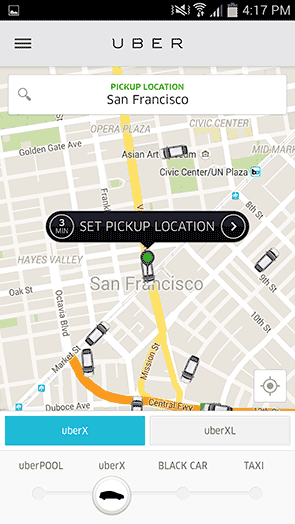
\includegraphics[scale=0.6]{imagens/uber.png}
	\caption{\small Interface principal do Uber Mobile.} Fonte: Referral SaaSquatch \cite{uber-imgs}
	\label{fig:uber-main-interface}
\end{figure}

\begin{figure}[H]
	\centering
	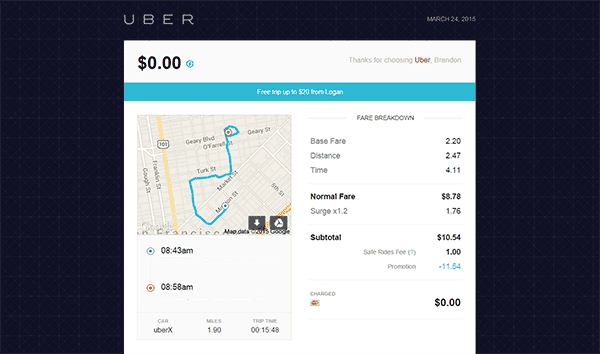
\includegraphics[scale=0.7]{imagens/uber2.png}
	\caption{\small Interface de pagamento do Uber Web.} Fonte: Referral SaaSquatch \cite{uber-imgs}
	\label{fig:uber-payment-interface}
\end{figure}

\section{Redis Publish-Subscribe (RedisMVA) }
Esta publicação \cite{redis-pubsub-redismva} faz parte de um projeto demonstrativo da utilização do padrão de comunicação pub/sub (Publish/Subscription), com um banco de dados NoSQL, chamado Redis. É abordada a implementação em NodeJS de um \textit{chat} de comunicação por texto, utilizando o padrão pub/sub para realizar a comunicação entre processos, onde os processos são as diversas instâncias que podem ser executadas de um mesmo servidor NodeJS distribuídos em diversos locais na internet.

O estudo desta publicação serviu como grande base de aprendizado para a elaboração da arquitetura do sistema que desenvolvemos, pois utilizava tecnologias atuais e que já tínhamos como plano para a implementação do nosso sistema, como citamos no caso do Uber. A utilização da linguagem de programação JavaScript, naturalmente traz um certo intimismo para quem já desenvolve para a \textit{web}, dado que ela pode ser considerada a linguagem da \textit{web} (\textit{client-side}), pois todos os maiores navegadores \textit{web} \cite{browsers-usage} utilizados no mundo interpretam a linguagem nativamente, sendo muito comum programadores voltados para a área já terem tido algum contato com a linguagem.

O autor da publicação disponibiliza todo o código fonte do projeto de demonstração com licença aberta, sendo assim, ele discorre sobre o tema de forma muito objetiva, apenas abordando em seu texto os pontos de interseção em que a implementação da comunicação pub/sub se insere. O texto oferece uma didática teórica de boa qualidade, demonstrando com diagramas e imagens da aplicação real, o funcionamento de cada passo do qual explica no documento.

A demonstração dos fluxos de dados que ocorrem no sistema ficam bem representadas com os diagramas, embora alguns destes fluxos não estejam implementados no sistema, como o balanceador de carga, visto que não era o foco de esclarecimento. É simples entender como a interface envia os dados para o servidor, que distribui os dados para os outros clientes conectados.

\section{Redis Pub-Sub (Rajaraodv)}
Esta publicação \cite{redis-pubsub-rajaraodv} fala sobre o mesmo assunto da citação anterior, que é a implementação de um chat por texto utilizando NodeJS e banco de dados Redis, mas nesta publicação o autor é mais abrangente no quesito de infraestrutura e escalabilidade da aplicação, abordando todos os passos para uma implantação completa do sistema em um servidor.

O texto da publicação é muito explicativo, é possível até para os mais principiantes no assunto de aplicações de tempo real entenderem a implementação e a finalidade de cada passo relatado. O texto também conta com ilustrações dos fluxos de dados na aplicação e demonstrações do funcionamento da interface.

O que se pode extrair do conteúdo desta publicação além da anterior, é a implementação do balanceador de carga, em conjunto com o \textit{proxy} reverso Nginx (aplicação que controla como será feito o fluxo de dados de fora para dentro da rede de servidores), o conceito de \textit{sticky sessions} (técnica que grava nas requisições de um cliente informações sobre servidor de origem da sessão) para traçar requisições a um mesmo servidor, e a integração do sistema em um servidor na nuvem (conjunto de recursos computacionais na internet, dedicados a hospedar aplicações de diversos tipos). 

Após o estudo da publicação deste autor, utilizamos em nossa implementação a utilização do Nginx. Entendemos a ideia de centralizar a distribuição de conteúdo estático da aplicação, como a interface, e canalizar as conexões aos servidores através de um ponto em comum, facilitando assim o gerenciamento para futuras implementações de \textit{sticky sessions}, balanceamento de carga, reconexão em casos de \textit{scale-up} ou \textit{scale-out} dos servidores (aumento e diminuição do número de servidores), entre outros benefícios que este tipo de arquitetura pode prover para as aplicações modernas. Tudo isso aspira o rumo em que a tecnologia vem tomando com o crescimento exponencial de usuários, consumo de dados, globalização, entre outros, que contribuem para a necessidade de se construir sistemas que sejam distribuídos e escaláveis, alcançando altos desempenhos.

\section{FanMappr e RadiusIM}
O FanMappr \cite{fanmappr} e o RadiousIM \cite{radiusim} são aplicações baseadas em \textit{chat} por localização geográfica, mas que foram disponibilizadas como produto, com a proposta de criarem relações sociais através da busca de usuários por localização, ou seja, são redes sociais e tinham isso como proposta final. Após uma análise mais técnica nos dois últimos tópicos em relação ao desenvolvimento da aplicação, agora iremos analisar ferramentas que implementam como um produto, aplicações que tem funcionalidades semelhantes as do nosso projeto.

Encontramos o FanMappr e RadiusIM após algumas poucas pesquisas que buscavam especificamente produtos que tivessem funcionalidades muito próximas das que implementamos em nossa aplicação. O FanMappr é uma aplicação com interface e funcionalidades aparentemente modestas, navegando entre os poucos menus que possui, percebemos que as funcionalidades se restringem somente ao \textit{chat} por texto e a um mapa terrestre onde os usuários são localizados.

A imagem \ref{fig:fanmappr-principal} é uma captura de tela da aplicação \textit{web} do FanMappr. Nela é possível notar a simplicidade da aplicação, que não possui personalizações das ferramentas utilizadas, como o mapa, e não utiliza conceitos de responsividade, pois a captura de tela foi realizada em um monitor de 22 polegadas, e a interface da aplicação se manteve no mesmo formato utilizado para tela menores.

\begin{figure}[H]
	\centering
	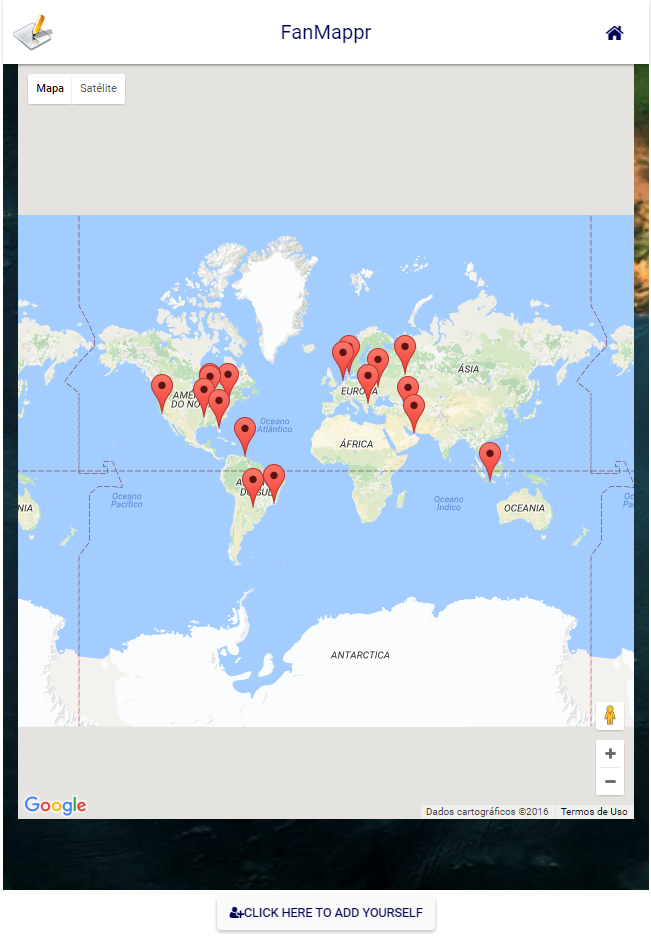
\includegraphics[scale=0.33]{imagens/fanmappr.png}
	\caption{\small Interface principal do FanMappr.} Fonte: Captura de tela
	\label{fig:fanmappr-principal}
\end{figure}

O RadiusIM não está mais disponível para acesso, mas encontramos um artigo \cite{radiusim} que possuía algumas imagens sobre a aplicação e uma breve explicação do seu funcionamento.

Foi possível notar que o RadiusIM também é muito semelhante com do FanMappr, apesar de parecer ter tido mais sucesso, nos anos 2000, presume-se que teve um investimento maior, pois possuía uma interface mais harmoniosa e funcionalidades que eram o de se esperar para sua época.

Podemos observar nas imagens \ref{fig:radiusim-principal} e \ref{fig:radiusim-chat} alguns detalhes de sua interface que demonstram um pouco da utilização do sistema. A imagem \ref{fig:radiusim-principal} \t mostra que de forma amigável ao usuário, a interface fornece os dados de sua localização, marcação no mapa, e uma série de pessoas nas proximidades e suas respectivas imagens de perfil. Na imagem \ref{fig:radiusim-chat} podemos ver a janela de chat 

\begin{figure}[H]
	\centering
	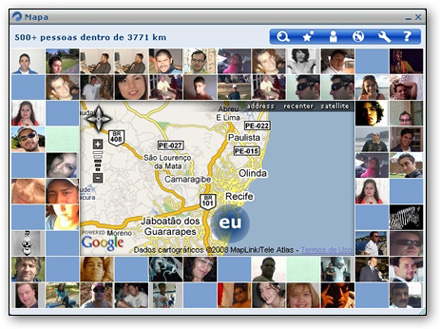
\includegraphics[scale=0.9]{imagens/radiusim.jpg}
	\caption{\small Interface principal do RadiusIM.} Fonte: wwwhats new \cite{radiusim}
	\label{fig:radiusim-principal}
\end{figure}

\begin{figure}[H]
	\centering
	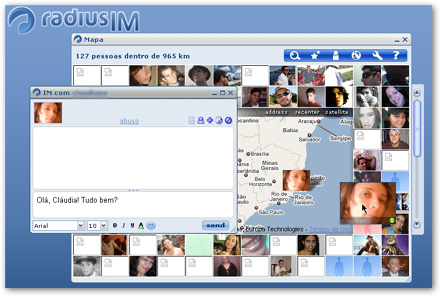
\includegraphics[scale=0.9]{imagens/radiusim2.jpg}
	\caption{\small Janela de \textit{chat} do RadiusIM.} Fonte: wwwhats new \cite{radiusim}
	\label{fig:radiusim-chat}
\end{figure}

É interessante perceber que estas aplicações não tiveram grande sucesso colocando como produto final uma ferramenta de comunicação com funcionalidades semelhantes a que iremos implementar, o que nos leva a interpretar que a \textit{web} em tempo real não é uma inovação a qualquer custo. É importante considerar que as melhorias que se pode ter com informações em tempo real devem ser mensuradas, e ela é apenas mais uma opção que está ganhando mais importância com as demandas que estão surgindo.

\section{Snapchat, Happn, Tinder e afins}
Neste tópico iremos fazer uma análise, mais filosófica do que técnica, sobre a utilização de aplicações de tempo real na vida dos usuários, pois achamos interessante fundamentar onde estão se rompendo os limites para a necessidade de aplicações deste tipo, e gostaríamos de ressaltar que Snapchat \cite{snapchat}, Happn \cite{happn} e Tinder \cite{tinder} foram escolhas que achamos que representam um grupo de aplicações com características próximas, mas que para muitas outras aplicações existentes, caberiam-se a mesma análise.

A seguir foi feita a síntese de uma citação \cite{notnotcitricsquid} que nos traz algumas importantes informações sobre a opinião de um usuário comum:

\begin{quote}
	\small "Há uma diferença fundamental entre chat baseado em localização e aplicativos de chat, como o Snapchat. O Snapchat mudou como as pessoas se comunicam, não mudou como elas encontram as pessoas para se comunicar.
	
	A localização em si não define quem somos ou o que gostamos, as pessoas buscam se comunicar com pessoas que possuam outros tipos de afinidades, e estas é que devem ser exploradas para se criar um aplicativo que seja interessante." 
	
	(Síntese de "Do location based chat apps start trending again?" \cite{notnotcitricsquid}, NOTNOTCITRICSQUID, 2012)
\end{quote}

A resposta a pergunta do tópico expressa uma opinião que condiz com alguns pontos que pudemos notar ao longo do conteúdo apresentado até aqui, que se relacionam com como as aplicações tem obtido sucesso na inserção da experiência de tempo real na vida dos usuários mais comuns, e aplicações como o FanMappr e o RadiusIM não alcançaram o mesmo resultado. Snapchat, Happn e Tinder são aplicações que utilizam localização geográfica em muitas de suas funcionalidades, mas trabalham a experiência do usuário com este tipo de funcionalidade de uma forma que preserva conceitos como os abordados na citação anterior, e este é um ponto que acreditamos ser o diferencial para a aceitação das ferramentas deste tipo, pelo fato de não infringir algumas barreiras que existem na interação humana com o mundo virtual.
	\chapter{Problematização}
\section{Caracterização do Problema}
A internet oferece diversas possibilidades de integração e distribuição de dados em sua rede mundial. A necessidade cada vez maior de se coletar dados que são gerados a todo momento, cria a iniciativa de se laborar novas maneiras de envio e recepção de dados na rede.

A transmissão de dados em tempo real não é uma necessidade recente, desde que se começaram a desenvolver sistemas críticos de controle na \textit{web}, muitos destes já utilizavam desta forma de se transmitir dados para realizar suas tarefas. As técnicas e tecnologias utilizadas para alcançar tal feito eram diferentes e mais custosas, o que levava este tipo de característica da aplicação ser adotada apenas em casos específicos, onde deveria se contrabalancear com mais perícia a utilização.

Com os avanços das tecnologias de \textit{hardware}, \textit{software} e da internet como um todo, começaram a se criar novas possibilidades da implementação de \textit{features} tempo-real em aplicações cada vez mais próximas do usuário comum. Com tudo isso, podemos observar que muitas das aplicações de sucesso do mercado usufruem desta tecnologia, que permite uma conexão direta e persistente entre cliente e servidor, viabilizando que se possa receber e enviar dados a qualquer momento, atualizando em tempo real todos os interessados em uma determinada informação.

A possibilidade da informação instantânea tem muito a contribuir em diversas áreas, oferecendo vantagem competitiva para quem está no mundo dos negócios, antecipação de tomada de decisões, entre outros benefícios. Este mundo do tempo-real está a cada vez mais tomando conta do nosso presente como usuários comuns, e a tendência é que essa forma de compartilhamento instantâneo se torne mais natural.

Como as pessoas utilizam e disponibilizam dados, tem uma importância fundamental no impacto em que isso pode ter em suas vidas. Desde as necessidades no mundo dos negócios, às necessidades do cotidiano de cada um. Por parte de quem está inovando no setor, é preciso entender comportamentos e como não romper barreiras que irão fracassar a relação entre tecnologia e pessoas. 

A implementação de funcionalidades tempo-real definitivamente se tornou algo exequível para as aplicações atuais na \textit{web}, como \textit{push notifications} (notificações de eventos que são emitidas do servidor para o cliente), \textit{stats} (status de dados), interações em jogos de navegadores, entre outros. Os \textit{WebSockets} funcionam analogicamente como os \textit{sockets}, e nos permite fazer a comunicação entre processos através da rede. Como o próprio nome diz, os \textit{WebSockets} são especificamente feitos para este tipo de comunicação na \textit{web}, possibilitando uma conexão contínua entre códigos JavaScript executados nos \textit{browsers} e os servidores \text{web}. Estes serão base fundamental para a resolução do problema proposto neste trabalho, levando em conta que são a tecnologia mais atual.

\section{Solução Proposta}
Buscando explorar a usabilidade tempo-real na \textit{web}, iremos formular nossa solução no desenvolvimento de uma aplicação de comunicação por texto, também podendo ser chamada de \textit{chat}. Para que os usuários tenham conhecimento da existência um do outro na aplicação, existirá um mapa terrestre do mundo real que será marcado com pontos identificadores de cada usuário utilizando o sistema. Estes pontos terão como base a coordenada geográfica real do usuário que será fornecida quando o usuário entrar no sistema.

A escolha por uma aplicação deste modelo se deve a ideia de querer tornar o entendimento do emprego da tecnologia mais amigável para as pessoas que não possuem conhecimento técnico muito aprofundado. A troca mensagens explícita em uma conversa entre duas pessoas, essencialmente ilustra a ideia de transferência de dados em tempo real, e em conjunto com a localização geográfica, conseguimos dar um adendo de outra aplicação da tecnologia.

Iremos desenvolver uma interface com a pretensão de ser amigável ao usuário, utilizando conceitos de responsividade para a adaptação do conteúdo mostrado em telas de dispositivos diversos, inclusive móveis, tendo em vista que algumas estatísticas \cite{internet-traffic-stats1} apontam que dispositivos móveis já são responsáveis por pelo menos um quarto do todo o tráfego de dados gerado na internet, e com estimativas \cite{internet-traffic-stats2} \cite{internet-traffic-stats3} de aumento em cada ano. Mesmo não sendo o foco da aplicação ser um produto final, achamos que o aprendizado com este tipo de requisito seria conveniente. Em relação a organização da interface, a aplicação terá duas telas principais, sendo a primeira com as opções de cadastro através do fornecimento de alguns dados pessoais, e autenticação no sistema por \textit{e-mail} e senha. A segunda tela será o ambiente principal da aplicação, onde o usuário poderá navegar por um mapa terrestre em busca de marcações que identifiquem outro usuário, com o qual ele poderá interagir através de uma janela de \textit{chat} por texto que surge neste mesmo ambiente.

O principal componente da solução será o servidor da aplicação. Este será desenvolvido sobre a arquitetura REST (Representational State Transfer), que transmite e recebe dados da interface no formato JSON (JavaScript Object Notation). Funcionalidades como cadastro de usuário e autenticação farão uso deste modelo. A comunicação tempo-real será provida por um \textit{framework} que utiliza como base a tecnologia de WebSockets para conexões bidirecional de dados entre servidor e cliente. Apesar da tecnologia WebSocket ser a mais apropriada para a este tipo de conexão, o próprio \textit{framework} trata de usar outras técnicas de comunicação tempo-real, como \textit{long polling}, em casos de falta de compatibilidade dos navegadores com a tecnologia de WebSocket. Tudo isso acontece de forma transparente ao usuário e ao desenvolvedor, pois a utilização do \textit{framework} se dá através de API (Application Programming Interface) que oferece de forma simplificada todo o processo de conexão e comunicação.

A persistência dos dados será feita através de um banco de dados no NoSQL. A escolha por este tipo de banco de dados se deve as características da aplicação que exigem muitas operações de I/O (Input/Output) em dados com baixo nível de relacionamento com outros dados, onde este tipo de tecnologia NoSQL oferece melhor desempenho e praticidade.

A tecnologia utilizada como ambiente de execução no servidor, utiliza o JavaScript como linguagem padrão, além de oferecer características que também beneficiam o tipo de aplicação que iremos desenvolver, como \textit{single-theaded} (aplicação executada em apenas uma thread, processando um comando por vez), \textit{non-blocking IO} (operações de escrita e leitura de dados não bloqueiam a execução de código) e \textit{asynchronism} (não existe ordem de execução dos blocos de código). 

Considerando também alguns conceitos de infraestrutura, iremos adotar na arquitetura da aplicação algumas formas de permitir o escalonamento dos serviços através da distribuição dos servidores em diversas instâncias no mesmo servidor físico ou em outros de locais distintos. Para isso utilizaremos tecnologias para fazer a comunicação entre processos, com um banco de dados NoSQL centralizado e em memória, e interações \textit{stateless}, onde o servidor não guarda dados de sessão do usuário.
	\chapter{Hardware e Software Utilizados}

\section{Codificação e Testes}
\subsection{Ambiente de Desenvolvimento}
O ambiente para desenvolvimento da solução foi criado em um único computador, de caráter pessoal, do tipo notebook, com as seguintes especificações técnicas \cite{notebook-info}:
	\begin{itemize}
		\item Processador Intel Core i5 3230M - 2.60 GHz (T-Max: 3.20 GHz) - 64 Bits - Smart Cache 3 MB L3
	\end{itemize}
	\begin{itemize}
		\item Chipset Intel ® HM75 Express
	\end{itemize}
	\begin{itemize}
		\item Memória RAM 8 GBs DDR3 SDRAM - 1600 MHz
	\end{itemize}
	\begin{itemize}
		\item Disco rígido 500GB - 5.400 RPM
	\end{itemize}
	\begin{itemize}
		\item Rede 10/100 e Wireless 802.11 b/g/n - Link de conexão com a internet de 15 Mbps
	\end{itemize}

Especificamos apenas algumas informações que julgamos serem de relevância para alguma análise de desempenho da aplicação por parte do leitor. Em nossa solução não iremos realizar levantamentos de dados sobre desempenho, pois este não pode ser considerado um ambiente que simule a realidade em servidores de aplicações, do qual seria de relevância este tipo de medição.

O sistema operacional escolhido para nosso ambiente de desenvolvimento foi o CentOS 7. O CentOS é uma distribuição Linux baseada no Red Hat. A Red Hat é uma empresa privada, que possui um O.S. chamado Red Hat Enterprise Linux (RHEL), e tem como proposta oferecer produtos \textit{enterprise} baseados no GNU/Linux. Tendo em conta que toda distribuição baseada no \textit{core} do Linux deve seguir uma série de regras contidas em sua licença, a Red Hat concentra seus faturamentos em suporte as distribuições que ela construiu. Ter um sistema compatível com o RHEL traz alguns benefícios que ainda não foram alcançados sem que se tenha um time de pessoas dedicadas ao desenvolvimento de um \textit{software} específico, como no caso da maioria dos sistemas open-sources, que é o alto padrão em testes contra erros e problemas de segurança, \textit{releases} mais curtos, correções de problemas em curto prazo, entre outros benefícios que o CentOS consegue absorver da comunidade Red Hat. Além disso, o CentOS já possui uma considerável comunidade ativa, que facilita na resoluções de problemas mais específicos e no desenvolvimento de novas funcionalidades. O sistema também já possui grandes \textit{cases} de sucesso, como Facebook \cite{facebook-distro} e Google \cite{google-redhat}, o que passa uma maior confiança para a adoção em outros negócios e uma perspectiva de crescimento contínua.

\subsection{Versionamento de Código}
O versionamento de código é uma tecnologia que permite traçar históricos de mudanças nos arquivos de código escrito através de um gerenciamento multi-usuário. Este gerenciamento permite que uma ou mais pessoas possam modificar um ou mais arquivos simultaneamente ou não, sendo controlados através de funcionalidades que permitem junção, revisão de conflitos, entre outros.

A tecnologia utilizada para versionamento de código neste projeto foi o Git. Este é um sistema de versionamento distribuído que atende a diversos tipos de \textit{workflows} de trabalho. A escolha por esta tecnologia se deve ao fato de ser umas das mais difundidas no mercado, e onde se encontram os maiores e mais confiáveis repositórios de código. Embora o fluxo de desenvolvimento tenha sido muito simples, utilizamos um \textit{workflow} chamado \textit{Gitflow Workflow} \cite{gitflow} que divide o desenvolvimento basicamente em dois \textit{branches} principais, um de produção e outro de desenvolvimento, podendo ser criado \textit{branches} de cada \textit{feature} sobre o \textit{branch} de desenvolvimento. 

\subsection{Editores de Texto}
Para o desenvolvimento majoritário do \textit{frontend}, utilizamos o editor de texto SublimeText 3 \cite{sublime}, apoiado de alguns \textit{plugins} para auxílio de escrita e design, como Emmit, ColorHighlighter, AlignTab, JSHint, MaterialTheme entre outros, todos podendo ser encontrado no repositório de pacotes packagecontrol.io \cite{packagecontrolio}.

Para o desenvolvimento do \textit{backend} e parte do \textit{frontend}, utilizamos o editor de texto Visual Studio Code 1.6 \cite{vscode}. A escolha por este outro editor de texto se fez principalmente pela funcionalidade de \textit{debug}, que apresentou melhores resultados em sua utilização, além de ser uma funcionalidade nativa da aplicação, assim como a ferramenta para versionamento de código. Também foi utilizado \textit{plugins} semelhantes aos escolhidos no SublimeText para auxílio de escrita de código, todos encontrados no repositório de pacotes padrão do editor.

\section{Back-end}
\subsection{NodeJS}
O NodeJS \cite{nodejs} é uma plataforma de desenvolvimento de alta performance construída sobre a \textit{Chrome's Javascript runtime V8} \cite{v8}. A V8 é um interpretador Javascript \textit{open source} desenvolvido em C++ pela Google e capaz de executar em sistemas operacionais Windows, Linux e iOS, consequentemente trazendo esta possibilidade de multi plataforma para o NodeJS. Comparando-se a uma tecnologia que está a mais tempo no mercado e se possui um maior entendimento, o funcionamento da \textit{engine} V8 é superficialmente semelhante ao fluxo de execução do conjunto JVM e JRE do Java.

A plataforma NodeJS possui uma arquitetura de funcionamento \textit{single-threaded} com operações orientadas a eventos e I/O não-bloqueantes. A escolha pela linguagem Javascript se molda bem a este tipo de funcionamento, pois por ser uma linguagem dinâmica e trazer características da programação funcional, como \textit{first-class functions} e \textit{function composition}, que auxiliam fortemente no controle do fluxo de execução através \textit{callbacks}, tornam a programação assíncrona mais fácil na plataforma, contribuindo para a criação de sistemas escaláveis e distribuídos.

Para um melhor entendimento de como o NodeJS trata as requisições feitas ao servidor, a imagem a seguir ilustra simplificadamente o fluxo de tratamento de uma requisição:

\begin{figure}[!htb]
	\centering
	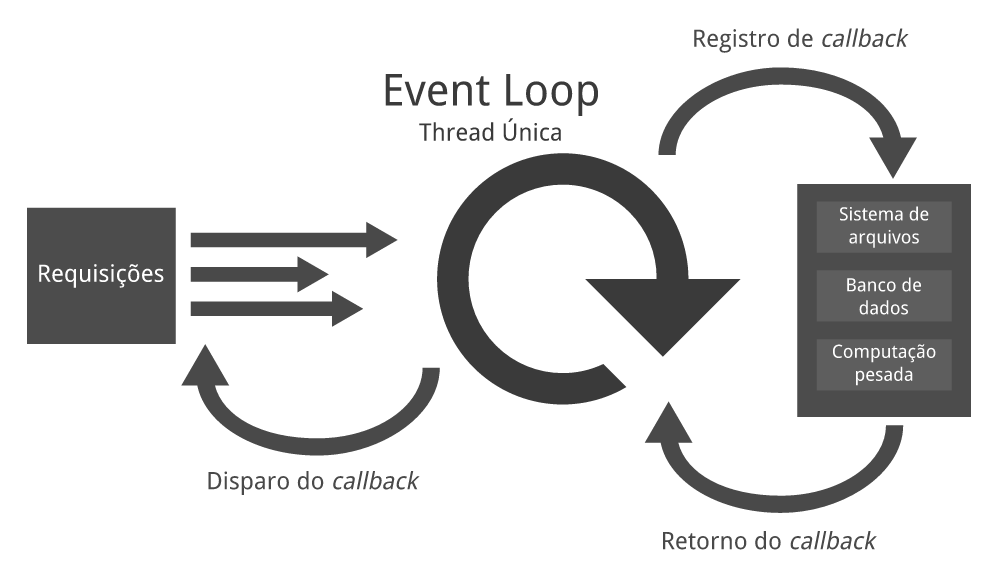
\includegraphics[scale=0.6]{imagens/node-eventloop.png}
	\caption{\small Fluxo simplificado de requisições no NodeJS. Fonte: maxroecker \cite{img-eventloop}}
	\label{fig:node-eventloop}
\end{figure}

Como se pode observar na figura, diferentemente dos servidores \textit{web} comuns, o NodeJS não cria um processo ou \textit{thread} para cada requisição que chega ao servidor. Ao invés disso, cada instância NodeJS é um processo que funciona como um \textit{event loop}, onde para cada operação de I/O requisitada, é registrada uma \textit{callback} que será chamada posteriormente no \textit{event loop} quando os dados estiverem disponíveis. Sendo assim, a thread principal nunca fica bloqueada, ela está sempre aguardando que um evento esteja para acontecer, que pode ser a chegada ou resposta de uma requisição, por exemplo. É possível que surjam questionamentos sobre como o NodeJS faz as requisições de I/O assíncronas e simultaneamente atende outras requisições, mas isso é abstraído ao desenvolvedor, pois o NodeJS utiliza um biblioteca multi-plataforma, codificada em C, chamada libuv \cite{libuv}, que trata as operações de I/O assincronamente com utilização de \textit{thread pool} e afins.

Tendo em mente todos esses conceitos do funcionamento da arquitetura do NodeJS, é possível entender o porque dele conseguir tratar muito mais conexões simultâneas do que as arquiteturas convencionais, pois a criação de processos e \textit{threads} tende a ser um recurso custoso para o sistema operacional, além de reservas de recursos valiosos do sistema, como memória RAM. É importante ressaltar que a programação assíncrona e o ambiente criado pelo NodeJS tem uma curva de aprendizado maior e se faz necessário maiores cuidados por parte do desenvolvedor, pois a utilização incorreta poderá acarretar no travamento da única \textit{thread} da instância da aplicação, bloqueando totalmente o sistema de processar novas requisições. 

Por outro lado, quando o entendimento é claro e o desenvolvimento é correto, a utilização dos recursos naturalmente é escalável e distribuída, pois a própria singularidade da plataforma nos faz trabalhar conceitos de sistemas distribuídos, como por exemplo, para que possamos aproveitar de todos os recursos de um processador multi-core com NodeJS, temos que executar mais de uma instância da aplicação, o que nos leva a trabalhar conceitos de clusterização, comunicação de processos e etc, o que facilita no escalonamento horizontal da aplicação em múltiplos servidores.

\subsection{NPM}
O NPM \cite{npm} é o gerenciador de pacotes do NodeJS. A função do NPM é oferecer um repositório central de qual se pode baixar diversos módulos distribuídos pela própria equipe que desenvolve o NodeJS ou que outros usuários tenham contribuído.

A evolução do NPM se tornou dominante, sendo considerado o maior repositório de registro de conteúdo Javascript do mundo. Devida a utilização do Javascript para outras finalidades além do desenvolvimento em NodeJS, muitos dos módulos disponibilizados pelo NPM não são parcialmente ou completamente desenvolvidos para a utilização com o NodeJS, sendo que muitos usuários e desenvolvedores utilizam e publicam conteúdo voltado para o desenvolvimento \textit{frontend}, que também utiliza o Javascript como principal linguagem. Talvez este seja um dos grandes motivos de sucesso do NPM em números.

Sua utilização é feita basicamente via linha de comando, onde iniciamos um novo repositório quando criamos uma aplicação, e apartir deste comando é criado um arquivo em formato JSON, chamado package.json, do qual ficará registrado todas as dependências daquele projeto, através da especificação do nome e versão de cada módulo baixado do repositório oficial.

A utilização de um gerenciador de pacotes traz diversos vantagens, dentre estas, a facilitação no versionamento de código, pois não é necessário manter uma cópia de um conteúdo que poderá ser baixado posteriormente de um local central, o controle das versões de cada biblioteca que se está utilizando no sistema, facilitando a resolução de problemas de compatibilidade e dependências uma das outras, local único para busca e contribuição de soluções na linguagem, entre outras.

\subsection{ExpressJS}
O ExpressJS \cite{expressjs} é o principal \textit{framework} NodeJS para desenvolvimento de aplicações \textit{web} e APIs. A sua proposta é ser simples, performático e \textit{loosely coupled} na construção de aplicações, sem interferir nas características padrões que o NodeJS oferece.

O desenvolvimento com o ExpressJS é bem intuitivo pela organização que ele propõe para a aplicação. Suas abstrações são apenas essenciais, que não interferem na utilização dos artifícios da própria linguagem nativa do NodeJS para a resolução dos problemas, sem muitas automatizações, sendo ainda mais conveniente oferecendo mecanismos de \textit{middlewares} que possibilitam total manipulação das requisições e seus atributos, injeção de \textit{template-engines} e outros \textit{handlers} e \textit{plugins} que podem ser baixados via NPM. A comunidade possui diversas soluções empregadas, o que também facilita na curva de aprendizado, produtividade e resolução de problemas. Rapidamente é possível instalá-lo na aplicação e se disponibilizar um servidor HTTP pronto para receber, tratar e responder requisições como API ou UI.

\subsection{SocketIO}
O SocketIO é uma biblioteca para a criação de aplicações tempo-real na \textit{web}, que permite troca de mensagens em formato binário ou texto de forma bi-direcional e instantânea. Ele funciona através de duas bases de código, uma aplicada no servidor NodeJS e outra no \textit{browser} do cliente. A biblioteca faz uso da tecnologia WebSocket para estabelecer uma comunicação bi-direcional e persistente entre servidor e cliente, mas em casos de problemas de compatibilidade, é utilizado o método de \textit{long polling} para estabelecer este tipo de comunicação. As bibliotecas do SocketIO utilizadas no servidor e no cliente possuem chamadas semelhantes, o que facilita na realização da interação dos dois lados.

A figura a seguir demonstra simplificadamente a forma de conexão entre servidor e cliente descrita anteriormente:

\begin{figure}[!htb]
	\centering
	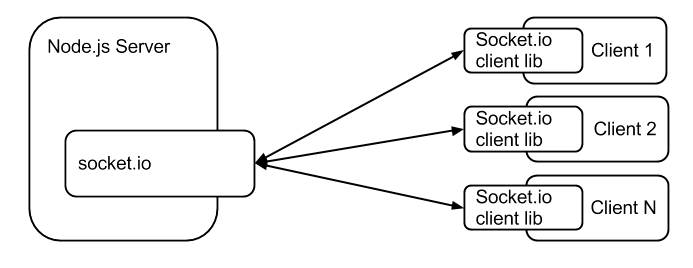
\includegraphics[scale=0.67]{imagens/socketio.png}
	\caption{\small Conexão entre servidor e cliente com SocketIO. Fonte: ifollow \cite{img-socketio}}
	\label{fig:socketio}
\end{figure}

Apesar do SocketIO ser um encapsulador da tecnologia \textit{websocket}, as chamadas de sua API são muito semelhantes a utilização do \textit{websocket} diretamente, onde a biblioteca apenas adiciona funcionalidades que são convenientes para o gerenciamento das conexões dos \textit{sockets}, como \textit{broadcast} de mensagens, atrelar informações específicas do usuário de cada \textit{socket}, entre outros.

A tecnologia \textit{websocket} é baseada em canais TCP, o que significa que os dados trafegados por ele tem a garantia de ordem e não perca de informações, o que torna a comunicação mais confiável e capaz de atender um abrangente número de necessidades. Também é preciso levar em conta os custos que canais TCP podem ter dependendo do tipo de dados que se quer transmitir, onde apesar da possibilidade de transmissão de conteúdo binário por \textit{websockets}, muitas das vezes é mais eficiente a utilização de um canal UDP, como faz uso a tecnologia WebRTC, que é muito utilizada para \textit{streaming} de vídeos, por exemplo.

\subsection{MongoDB}
O MongoDB é um banco de dados de alta performance, enquadrado nos conceitos de bancos de dados NoSQL. A escolha por este tipo de ferramenta se faz pelas características que o modelo de arquitetura escolhido traz para a aplicação. Os bancos de dados NoSQL foram criados para oferecer novas possibilidades para as demandas que exigem escalabilidade horizontal e performance na estrita e leitura de dados, o que se encaixa com os atributos das tecnologias da aplicação desenvolvida.

A forma como este tipo de banco de dados funciona remete diretamente aos ganhos de desempenho e escalabilidade, pois existe uma quebra de conceitos dos bancos de dados relacionais, como o ACID, que trazem flexibilidade em como se tratam os dados armazenados para se ter os benefícios citados. O MongoDB além de adotar estes conceitos, é um banco de dados orientado a documentos, onde a persistência dos dados é realizada em formato JSON. Apesar do conceito NoSQL ser uma grande ruptura de paradigmas, a maior parte da popularidade do MongoDB se deve a sua forma de interação com o usuário, que é amigável a quem está migrando dos conceitos relacionais para o modelo NoSQL. Apesar de não existir a necessidade de criação de tabelas, definição de relações, entre outros, a API do MongoDB oferece a criação de esquemas que remetem a conceitos parecidos, e também habilitam outras possibilidades, como a indexação de campos para buscas mais eficientes. As chamadas de busca no banco também são amigáveis, utilizando palavras chaves como \textit{SELECT, WHERE, ORDER BY}, entre outros. É importante salientar que algumas das funcionalidades citadas se devem ao uso de um modelador de dados chamado Mongoose \cite{mongoose}, ferramenta da qual oferece um \textit{set} de utilidades para se trabalhar com o MongoBD.
 
\subsection{Redis}
O Redis é um banco de dados NoSQL em memória, que implementa apenas alguns tipos de estruturas de dados, como \textit{strings, hashes, lists, sets} e \textit{sorted hashes}, e funcionalidades para gerência, busca e transmissão dos dados armazenados, o que o torna muito enxuto. Devido ao Redis ser um banco de dados que funciona em memória, seu desempenho é muito alto, tendo em vista que a memória RAM é um dos componentes de armazenamento de dados mais rápidos em leitura, escrita e transmissão na arquitetura computacional. Por outro lado, a memória RAM é volátil, o que nos leva a buscar entender qual a proposta de um banco de dados em memória.

A utilização principal do Redis é para servir como \textit{cache} e/ou \textit{message broker} de informações em sistemas. Em implementações \textit{stateless} o Redis pode servir como \textit{cache} de dados muito requisitados, pois seu rápido desempenho em memória pode ser vital para atender requisições em tempo hábil. Outra utilidade do Redis, que é o caso deste projeto, é do compartilhamento de dados entre servidores distintos de uma aplicação, onde através das estruturas de dados fornecidas pelo Redis e algumas funcionalidades, como a do protocolo PUB/SUB, é possível que se armazene dados no Redis e outra instância da aplicação sendo executada em outro local possa buscar estes mesmos dados. Devido a simplicidade e robustez que o Redis possui, uma única instância é capaz de realizar milhares de operações, aproximadamente 1.5 milhões por segundo \cite{redis-metrics}, podendo funcionar muito bem sendo este tipo de centralizador, pois o escalonamento de servidores de aplicação ocorre com muito mais frequência do que a de instâncias Redis. 

\section{Front-end}

\subsection{Bower}
O Bower \cite{bower} é um gerenciador de pacotes, assim como o NPM, mas com conteúdo focado para o \textit{frontend}. Através dele é possível fazer \textit{download} de diversas bibliotecas, como AngularJS, jQuery e Bootstrap. Sua utilização se dá através de linha de comando, onde ao criar um novo projeto \textit{frontend} o usuário deve iniciar o Bower no mesmo diretório, através de linha de comando, e este criará um arquivo chamado bower.json, que conterá informações do projeto e todas os nomes e versões de bibliotecas baixadas do seu repositório oficial, permitindo-se assim o gerenciamento de novos pacotes e resolução de dependências entre eles.

O NPM também oferece muitas das bibliotecas disponíveis no Bower, e o contrário muitas vezes não é válido, sendo assim, é comum a utilização dos dois gerenciadores de pacotes no projeto \textit{frontend}, o Bower e NPM.

\subsection{AngularJS}
O AngularJS \cite{angular} é um \textit{framework} Javascript para desenvolvimento de interfaces \textit{web}. Mais do que apenas interfaces, o AngularJS auxilia na criação de aplicações complexas no lado cliente da comunicação. Com o avanço das tecnologias e formas de se construir sistemas, ferramentas como o AngularJS vieram para ajudar na organização e qualidade dos sistemas que estavam se desenvolvendo.

A abordagem do AngularJS na construção de aplicações \textit{frontend} é completa, oferecendo suporte para manipulação do DOM, \textit{data binding}, gerenciamento de rotas, padrões de projeto (MVW, MVVM, MVC), entre outros. Apesar da fragmentação de alguns recursos em módulos separados, como as rotas, o produto AngularJS consegue oferecer uma solução completa para o desenvolvimento de interfaces de usuário.

O desenvolvimento de uma aplicação AngularJS, normalmente segue as diretivas de uma aplicação SPA com o estilo de programação declarativa, tendo em vista a forma com que se desenvolve interfaces para os \textit{browsers}, as tecnologias envolvidas, como o próprio HTML, em um ambiente orientado a eventos, se faz mais adequada este tipo de abordagem declarativa, que segue uma lógica mais comum as interfaces.

A arquitetura moldada ao um formato de API também é um fator determinante para a utilização de um \textit{framework} como o AngularJS, pois ele já oferece módulos e serviços para o consumo de dados através de \textit{endpoints} que forneçam dados em formato XML ou JSON.

\subsection{Angular Material}
O Angular Material \cite{angular-material} é uma outra solução do produto Angular, também para interfaces, mas focado em conceitos e características de \textit{design}, UX, reutilização, acessibilidade, compatibilidade \textit{cross-browsers}, responsividade, entre outros. 

A ferramenta oferece diversos componentes visuais de interface com efeitos e estilizações próprios, levando em conta diversos conceitos abstratos de \textit{design}, que enriquecem a experiência e agradabilidade do usuário ao ver e interagir com eles. Os componentes do Angular Material são totalmente compatíveis com as implementações AngularJS, facilitando na integração entre os componentes. Um grande problema que é evitado utilizando um \textit{framework} como este, são os de problemas de compatibilidade entre os diversos navegadores no mercado, onde cada um possui especificidades que podem causar comportamentos inesperados nos comentos de interface. Acessibilidade e outras otimizações também são importantes para a inclusão do site e SEO.

Por último, um benefício importante que o Angular Material dispõe, é o seu \textit{grid system}, baseado no CSS3 \textit{flexbox}. Esta característica possibilita que todo o conteúdo apresentado no site se redimensione de acordo com o tamanho da tela do dispositivo que está exibindo o conteúdo, possibilitando assim uma experiência viável para dispositivos móveis, do qual já citamos a importância em números \cite{internet-traffic-stats1} \cite{internet-traffic-stats2} \cite{internet-traffic-stats3}.  

\subsection{Gulp}
O Gulp \cite{gulp} é uma ferramenta de automatização de tarefas Javascript, comumente utilizado para automatizações de fluxos de trabalho no desenvolvimento \textit{frontend}. Sua utilização se dá por linha de comando e um arquivo de configuração chamado gulpfile.js. Neste arquivo Javascript podemos criar \textit{tasks} que irão realizar tarefas diversas, de acordo com a programação realiza, como por exemplo a execução de testes unitários, concatenação e minificação de arquivos, compilação de linguagens intermediárias, como o SASS, \textit{autoprefixer}, \textit{lint}, entre outros.

Existem diversos \textit{plugins} disponíveis no NPM que executam tarefas específicas, como as citadas anteriormente, bastando ao usuário baixá-las e chamá-las em suas \textit{tasks}, que podem executar uma ou mais funcionalidades organizadas através de chamadas síncronas pelo método pipe de cada \textit{task}.

\subsection{SASS}
O SASS \cite{sass} é uma linguagem de \textit{script} que pode ser interpretada para CSS. O CSS tem uma sintaxe muito simples e com poucas funcionalidades para estruturação, reaproveitamento e modularizarão de código, onde o SASS oferece uma série de funcionalidades, como variáveis, operadores, herança e modularização, que podem ser aplicadas para a geração de folhas de estilos.

Todas as funcionalidades do SASS facilitam a construção de interfaces complexas, onde se exigem muitos componentes, classes, hierarquização de seletores, entre outros. A interpretação do código SASS para CSS pode ser feita por diversos interpretadores, inclusive o próprio Gulp oferece \textit{plugins} para este fim.

\subsection{HAML}
O HAML \cite{haml} é uma linguagem que tem a proposta de facilitar a escrita do HTML através de uma sintaxe mais curta, edentação de código e alguns conceitos de HTML dinâmico. Neste projeto utilizamos mais especificamente o HAMLJS \cite{hamljs}, que é uma derivação da versão principal do HAML, que habitualmente é utilizado com Ruby on Rails. Essa derivação do HAML oferece uma implementação em Javascript, assim possibilitando sua utilização em diversas ferramentas que utilizam a linguagem. O funcionamento do HAML é parecido com o do SASS e a interpretação dos arquivos HAML para HTML pode ser feita por diversas ferramentas, inclusive \textit{plugins} do próprio Gulp podem realizar esta tarefa.

Apesar da escolha de utilização de uma ferramenta transcrita de outra linguagem, existem diversas opções de \textit{template engines} feita exclusivamente para a utilização com Javascript, como o Jade e o EJS, e que podem trazer melhor qualidade das funcionalidades e \textit{releases} mais curtos com novas implementações.

\subsection{Webpack}
O WebPack \cite{webpack} é um Javascript \textit{module bundler}. Devido a linguagem Javascript não possuir um sistema para isolamento de escopo dos diversos blocos de código que podem existir em uma aplicação, o WebPack proporciona essa funcionalidade baseando-se nos principais padrões de módulos Javascript utilizados, como o AMD e CommonJS, onde ele é capaz de gerenciar todas as dependências entre módulos e gerar \textit{assets} estáticos para a utilização.

A utlização do WebPack se faz principalmente no desenvolvimento \textit{frontend}, pois o NodeJS, principal ambiente de desenvolvimento com Javascript do lado servidor, já adota o sistema de módulos CommonJS, o que aproxima ainda mais os conhecimentos de desenvolvimento \textit{frontend} e \textit{backend} com a adoção de módulos CommonJS nos dois lados, além dos benefícios na organização e isolamento de códigos. Também é possível a utilização de \textit{plugins} intermediários com o WebPack, estes podem oferecer diversas funcionalidades, como interpretação de ECMAScript 2015 ou TypeScript.

\subsection{Babel}
O Babel \cite{babel} é um compilador Javascript que permite a utilização das novas funcionalidades do ES2015. Devido a esta grande atualização do Javascript não ser compatível com uma grande maioria dos navegadores do mercado, o Babel oferece a opção de se escrever o código Javascript com a sintaxe ES2015 e ter a geração de outro arquivo traduzido para o ES5, que é a implementação com maior compatibilidade entre navegadores.

A utilização do Babel pode ser feita utilizando diversas ferramentas, como o Gulp ou o WebPack. Quando se utiliza o WebPack no projeto, é preferível que se faça a integração do Babel com ele, pois como ele cuida da resolução de dependências entre os módulos, ele consegue tratar no momento certo a tradução do código em ES2015 para ES5, evitando problemas de interpretação e compatibilidade. 

\subsection{Nginx}
O Nginx \cite{nginx} é um servidor \textit{web} de alta performance \textit{single-threaded}, uma arquitetura parecida com a do NodeJS, com funcionalidades que o permitem atuar como \textit{proxy} reverso e/ou \textit{load balancer} de aplicações. Para demonstrar onde o Nginx se encaixa na infraestrutura de uma aplicação \textit{web}, podemos observar a seguinte imagem:

\begin{figure}[!htb]
	\centering
	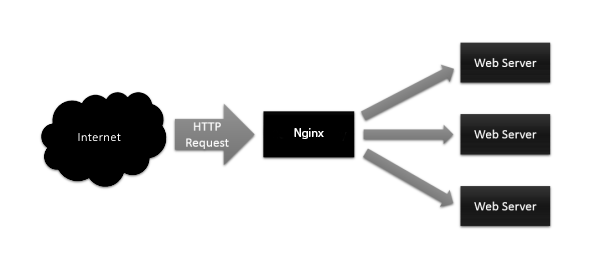
\includegraphics[scale=1]{imagens/nginx.png}
	\caption{\small Localização do Nginx na arquitetura de aplicações \textit{web}. Fonte: Thunder-Boy \cite{img-nginx}}
	\label{fig:nginx}
\end{figure}

O conceito de \textit{proxy reverso} se dá pela capacidade do Nginx encaminhar requisições de entrada para os servidores da rede privada, ao contrário do que ocorre com os \textit{proxys} comuns, que encaminham o tráfego de saída da rede. Sendo assim, o Nginx está na frente dos servidores de aplicação e gerencia todas as conexões que chegam de um determinado domínio, possibilitando assim que também gerencie controles de \textit{cache}, conexões SSL, \textit{streaming}, fornecimento de conteúdos estáticos da aplicação, como arquivos HTML, folhas de estilo, scripts, imagens, entre outros.

O Nginx também pode funcionar como um \textit{load balancer}, tendo em vista que ele recebe todas as conexões e conhece todos os caminhos para os servidores, bastando apenas a implementação de um ou mais algoritmos de balanceamento de carga, como Round Robin, Least Traffic, Least Latency, URL, entre outros. Uma funcionalidade importante que também pode ser implementada com a ajuda do Nginx é o conceito de \textit{sticky sessions}, que por exemplo, é uma opção para o funcionamento de conexões \textit{websockets} em aplicações distribuídas em múltiplos servidores, devido a necessidade de se manter as requisições traçadas ao mesmo servidor que contém suas informações de conexão.
	\chapter{Implementação}
A implementação do sistema segue todas as diretrizes de tecnologias e conceitos apresentados até este tópico. A descrição de como a implementação foi feita será dividida em duas partes principais: \textit{backend} e \textit{frontend}. Sendo a parte de \textit{backend} a implementação da infraestrutura e servidor da aplicação, e na parte do \textit{frontend} a implementação de interface com o usuário. No desenvolvimento elegemos um nome fictício para a aplicação, chamado Orb. Este nome será utilizado para remeter a aplicação em alguns textos, logos, implementações, entre outros.

\begin{figure}[!h]
	\centering
	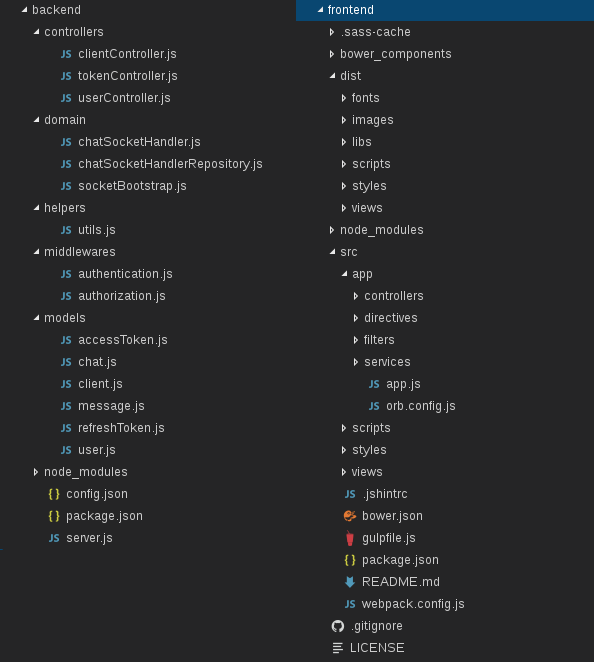
\includegraphics[scale=0.75]{imagens/estrutura_arquivos.png}
	\caption{\small Estrutura de arquivos do projeto.}
	\label{fig:estrutura-arquivos}
\end{figure}

O código-fonte da aplicação está hospedado no GitHub \cite{orb}, como \textit{software open-source}, liberado para utilização através da licença MIT \cite{mit}. A abordagem utilizada para a descrição da implementação feita fará referências pontuais a trechos do código-fonte que poderão ser consultados pelo leitor no repositório informado \cite{orb}, evitando-se assim a exposição de código neste formato de texto que não é favorável a análise deste tipo de conteúdo.

\section{Backend}
Primeiramente iremos descrever a criação do ambiente de desenvolvimento do projeto, onde inicialmente foi instalado o sistema operacional e todas as ferramentas que decidimos utilizar para a construção da aplicação, e posteriormente iniciamos o processo de codificação.

Iniciando-se pelo sistema operacional, foi criada uma partição separada no disco rígido, com volume de 60 GBs. O sistema operacinal escolhido para o ambiente de desenvolvimento foi de uma distribuição Linux chamada CentOS \cite{centos}, versão 7. A instalação do sistema operacional foi feita através de um \textit{pendrive} e foram seguidas todas as configurações padrões do \textit{wizard} de instalação do sistema.

Após a instalação do sistema operacional, foi feita a instalação de todas as ferramentas que foram escolhidas para o desenvolvimento da aplicação, como o NodeJS, MongoDB, Redis, editores de texto e navegadores. Todas estas ferramentas foram instaladas através do repositório de pacotes padrão do sistema CentOS 7, chamado YUM. Para algumas ferramentas foram necessário a atualização das fontes do repositório YUM e outras foram instaladas através de pacotes RPM (Red Hat Package Manager ou RPM Package Manager) disponibilizados no próprio site da ferramenta.

A implementação do \textit{backend} iniciou-se com a criação de um diretório chamado backend na pasta raiz do projeto, do qual a partir dele foram seguidas recomendações de boas práticas \cite{express-app-structure} para a organização da estrutura de diretórios em aplicações ExpressJS. A seguinte listagem identifica o nome destes diretórios e suas respectivas funcionalidades:

\begin{description}
	\item[controllers] Este diretório contém os arquivos de código relacionados as rotas e suas lógicas de implementação. Rotas são os \textit{endpoints} que podem ser acessados através de requisições HTTP enviadas por uma determinada URL que a identifica. Neste diretório contém os arquivos das rotas de cliente, usuário e \textit{token}.
	
	\item[domain] Este diretório contém os arquivos relacionados a lógica de negócio da aplicação. Os \textit{handlers} que tratam as requisições \textit{websocket} da aplicação estão implementados em arquivos contidos nesta pasta.
	
	\item[helpers] Este diretório contém arquivos que implementam funcionalidades que podem ser utilizadas em diversos pontos do sistema, este diretório funciona como um \textit{cross-cutting layer} da aplicação. Nesta pasta estão implementados alguns métodos que ajudam na geração de \textit{random strings} e retorno de \textit{datetime} em formato UTC (Coordinated Universal Time).
	
	\item[middlewares] Este diretório contém arquivos relacionados a \textit{middlewares} de tratamento de requisições que chegam ao servidor, como realização de autenticação e autorização de acesso as rotas da aplicação.
	
	\item[models] Este diretório contém arquivos relacionados aos objetos que podem ser persistidos na aplicação. Devido ao Javascript ser uma linguagem dinâmica, estes objetos não representam um contrato de como estes eles devem existir na aplicação, mas como eles devem ser persistidos no banco de dados, que no caso desta aplicação é o MongoDB. Neste diretório serão encontrados os arquivos de persistência dos \textit{tokens}, \textit{chat}, \textit{messages}, \textit{users}, entre outros.
\end{description}

Após a definição da estrutura de diretórios da aplicação, foi realizada a instalação e inicialização do NPM, responsável por gerenciar todos os pacotes que iremos utilizar no desenvolvimento da solução.

\subsection{Persistência}
A persistência dos dados foi feita em um banco de dados MongoDB, onde para sua utilização foi feito o \textit{download} doo pacote Mongoose pelo NPM. A conexão com o banco foi feita no arquivo de inicialização da aplicação, através do método connect do próprio Mongoose, passando-se como parâmetros uma \textit{connection string} com o endereço local do banco de dados. Por ser um ambiente de testes, não utilizamos autenticação com o banco de dados, mas caso fosse necessário, bastava-se apenas adicionar os dados de \textit{username:password} na própria \textit{connection string}.

No diretório \textit{models} foram criados arquivos para cada objeto que fosse ser persistido no banco. As implementações da persistência utilizaram o Mongoose como modelo, exportando de cada módulo o objeto \textit{schema} de cada persistência, podendo através deste realizar todas as operações de CRUD (Create, Read, Update, Delete).

A figura \ref{fig:modelsuml} ilustra a representação dos objetos persistidos no banco de dados:

\begin{figure}[!h]
	\centering
	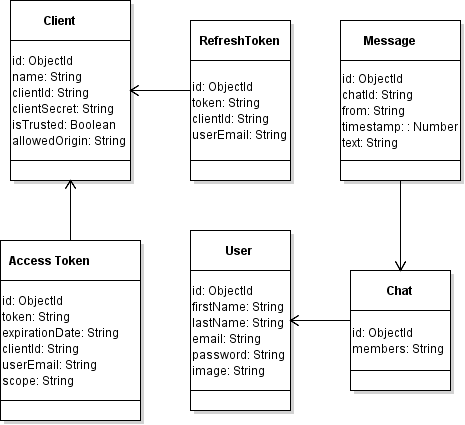
\includegraphics[scale=0.85]{imagens/models_uml.png}
	\caption{\small Representação UML (Unified Modeling Language) dos modelos persistidos no banco de dados.}
	\label{fig:modelsuml}
\end{figure}

\begin{figure}[!h]
	\centering
	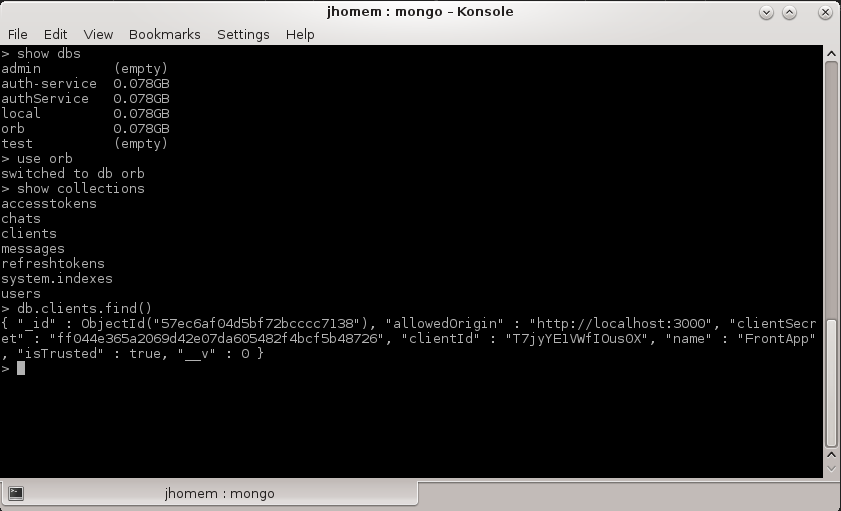
\includegraphics[scale=0.60]{imagens/mongo_console.png}
	\caption{\small Demonstração de utilização do MongoDB pelo terminal do CentOS.}
	\label{fig:mongoconsole}
\end{figure}


\subsection{Autenticação e Autorização}
Para a implementação do sistema de autenticação, cujos códigos estão no diretório middlewares, utilizamos três pacotes NPM, que funcionam como \textit{middlewares} que extraem de um \textit{request} as informações de autenticação, e através de uma \textit{callback} é possível validar essas informações e sinalizar se as informações estão corretas para concretização da autenticação. Para o sistema de autorização, utilizamos o OAuth2 com algumas modificações em seu padrão para atender aplicações \textit{trusted}, como o nosso \textit{frontend app} desenvolvido em AngularJS, que é um tipo de aplicação que não necessita de autorização do usuário da conta para acessar suas informações confidenciais.

Como estamos utilizando um sistema de \textit{tokens}, para realizar acesso ao \textit{endpoint} token, o qual é utilizado no sistema de \textit{login} para se conseguir um Access Token e um Refresh Token através do fornecimento de \textit{e-mail} e senha, é realizada a autenticação pelos padrões Basic \cite{passport-basic} e Client \cite{passport-client}. Após esta autenticação, o usuário é encaminhado para um \textit{exchange} do OAuth2 que irá gerar, persistir e retornar um Access Token e um Refresh Token para o solicitante, que poderá usá-lo para acessar os demais \textit{endpoints} da aplicação.

Como já introduzido, o restante dos das rotas da aplicação são protegidos através do padrão de autenticação Bearer \cite{passport-bearer}, que procura em cada requisição feita um Access Token, que será verificado, e caso seja válido permitirá o acesso ao \textit{endpoint} solicitado. Em caso do Access Token não ser válido, o servidor irá emitir uma resposta de erro, HTTP 401, informando o problema ocorrido, e se o problema for a expiração do Access Token, ele poderá utilizar o Refresh Token para conseguir um novo Access Token válido por mais um determinado tempo, evitando de ter que realizar toda o processo de autenticação com \textit{e-mail} e senha novamente.

\begin{figure}[!htb]
	\centering
	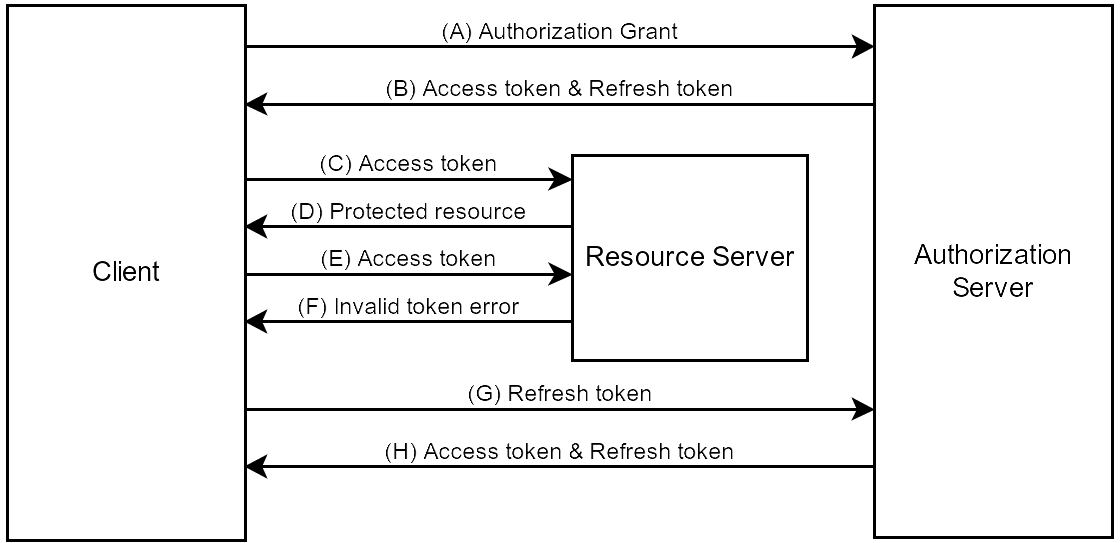
\includegraphics[scale=0.49]{imagens/oauth2.png}
	\caption{\small Fluxo de acesso aos recursos com OAuth2. Fonte: jlabusch \cite{img-jlabusch}}
	\label{fig:oauth2}
\end{figure}

Um detalhe importante que deve ser falado, é a utilização do método bcrypt \cite{bcrypt} para criptografia da senha dos usuários e a utilização do crypt \cite{crypt} para a criptografia do Access Token e Refresh Token. Como o bcrypt é um tipo de criptografia mais complexa, que leva em conta o custo de processamento, utilizamos-o em funcionalidades menos requisitadas, como o \textit{login}, e utilizamos o crypt (SHA256) para a criptografia dos \textit{tokens}, pois são requisitados na maioria das rotas do sistema, consequentemente necessitando-se fazer a verificação de chaves a todo momento, sendo assim, a utilização de um método menos custoso se faz benéfico.

\subsection{Rotas}
As rotas de aplicação estão organizadas no diretório controller da aplicação, tendo sido implementadas de acordo com o tipo de persistência que elas representam. A seguir, uma listagem organizada pelos \textit{endpoints} das rotas e uma descrição sobre sua funcionalidade:

\begin{description}
	\item[client] A rota client possui dois \textit{endpoints} que podem ser acessados através de chamadas pelo método HTTP GET e HTTP POST. O método GET retorna uma lista em formato JSON de todos os clients cadastrados no sistema. O método POST recebe um client em formato JSON e cadastra-o no banco.
	
	\item[token] A rota token possui apenas um \textit{endpoint} chamado revoke, o qual é responsável por remover do banco de dados o Access Token e Refresh Token relacionados a um determinado cliente. Este \textit{endpoint} é utilizado para realizar o \textit{signout} da aplicação.
	
	\item[user] A rota user possui quatro \textit{endpoints}, sendo o primeiro podendo ser chamado pelo método GET e retornando todos os usuários persistidos. O segundo pelo método GET, passando-se como parâmetro o id do usuário que se quer retornar. O terceiro pelo método POST, passando-se como parâmetro o usuário em formato JSON que se quer persistir. O quarto pelo \textit{endpoint} accesstoken e método GET, passando-se como parâmetro o Access Token do usuário que se quer retornar.
\end{description}

As rotas seguem o padrão de utilização dos métodos HTTP para realização do CRUD em APIs, sendo os \textit{endpoints} citados funcionalidades da aplicação, e são protegidos de acordo com as especificações faladas no tópico Autenticação e Autorização. Estes \textit{endpoints} são chamados pela aplicação \textit{frontend}, que passa em cada \textit{request} todas as informações de autenticação necessária, e trata os dados de sucesso ou erro que cada \textit{endpoint} retorna.

\subsection{Socket}
O desenvolvimento da comunicação em tempo real do \textit{chat} é a principal funcionalidade do \textit{backend} da aplicação. Os arquivos de implementação estão localizados no diretório domain, onde três arquivos implementam todas as funcionalidades relacionadas.

Inicialmente foi feito o \textit{download} pelo NPM das bibliotecas socket.io e redis. A inicialização do servidor de conexão do socket.io foi feita no arquivo de inicialização do servidor através da porta 1200. A conexão com o banco de dados Redis foi feita no arquivo que trava os eventos dos \textit{sockets}.

Com a biblioteca devidamente configurada, o servidor já está pronto para receber conexões \textit{socket}. No arquivo socketBootstrap.js criamos um sistema de inicialização que cria um \textit{namespace} de conexão chamado chat, e também realiza a autenticação dos usuários que tentam estabelecer uma conexão por \textit{socket} com o servidor. Para tratar a autenticação, utilizamos uma biblioteca \cite{socketio-auth} que oferece uma solução semelhante a explicada no tópico Autenticação e Autorização.

No arquivo chatSocketHandler.js implementamos todos os eventos de envio e recebimento de mensagens dos \textit{sockets}. Visando a utilização do protocolo PUB/SUB, abrimos três conexões/canais com o nosso servidor Redis, o primeiro para \textit{publish} de mensagens, o segundo para \textit{subcription} e o terceiro para \textit{storage} de informações dos usuários \textit{online}.

A seguir uma lista dos eventos emitidos e recebidos no \textit{namespace} chat e a descrição de seu funcionamento:

\begin{description}
	\item[disconnect] Este evento é emitido por um cliente que se desconectou do servidor. Neste evento tratamos de remover este usuário da lista de usuários \textit{online} do \textit{storage} e lançamos um evento chat:signout, comunicando a todos os usuários que aquele usuário se desconectou, logo devem o remove-lo de seu mapa.
	
	\item[chat:signout] Este evento é emitido para todos os usuários, informando-os o id de um usuário que acabou de se desconectar do servidor. Quando este evento é recebido pelo cliente, ele procura e remove este usuário do seu mapa.
	
	\item[chat:new] Este evento é emitido pelo cliente quando ele inicia um \textit{chat} com outro usuário. Este evento procura no banco de dados a existência de uma conversa entre os dois usuários, caso exista, esta conversa é lida com as últimas 15 mensagens registradas. Caso não exista, é criada uma nova conversa entre os usuários.
	
	\item[chat:online:list] Este evento é recebido pelo servidor e emitido por ele próprio com uma lista de informações de todos os usuários \textit{online}, inclusive suas respectivas localizações geográficas.
	
	\item[chat:message:send] Este evento é emitido pelo cliente quando ele clica no botão de enviar de um janela de \textit{chat}. Neste evento é enviado os dados do \textit{chat}, como a mensagem e o id do chat, e o \textit{handler} deste evento no servidor registra e mensagem no banco de dados e a envia para todos os membros da conversa.
	
	\item[chat:message] Todo cliente é capaz de receber este evento. Quando o servidor recebe um evento chat:message:send, ele registra a mensagem no banco e envia para cada membro do \textit{chat} a respectiva mensagem através deste evento.
	
	\item[chat:position:update] Este evento é emitido pelo cliente, com latitude e longitude de sua localização geográfica, quando ele se conecta ao \textit{chat} e quando ele se movimento pelo menos 100 metros em alguma direção. Após receber este evento o servidor emite o mesmo, juntamente com os dados do usuário para todos os outros clientes, assim eles podem atualizar a localização real do usuário em seus mapas.
	
	\item[chat:ready] Este evento é emitido pelo servidor para um usuário que acabou de se conectar após todos os eventos relacionados aquele a ele tenham sido registrados.
\end{description}

É importante frisar a emissão de eventos por parte do servidor são feitas através da função init, que é registrada quando se executa o servidor, onde esta função utiliza o sistema de PUB/SUB do redis para receber as mensagens, procurar a existência do \textit{socket} de destino em sua lista de \textit{sockets} conectados a aquele servidor, e se encontrado a mensagem é enviada a ele. Este esquema de funcionamento é que permite a comunicação entre os diversos servidores que a aplicação pode ter, pois todos os servidores irão receber uma mensagem publicada no Redis por algum deles, podendo assim verificar se a mensagem pertence a algum de seus clientes e enviá-la ou não.

Toda a interação com o banco de dados é feita através do repositório criado no arquivo chatSocketHandler.js. Neste arquivo estão implementados diversos métodos e serviços de CRUD para os eventos dos \textit{sockets}.

\section{Frontend}
O desenvolvimento da aplicação \textit{frontend} foi feito com AngularJS. O uso deste \textit{framework} trouxe para a aplicação algumas características importantes para a construção de interfaces, como o conceito de SPA e um padrão de projeto, que quando se lançou a ferramenta a documentação declarava este padrão como MVVA, mas ao longo do tempo os desenvolvedores foram adquirindo novas formas de se trabalhar com o AngularJS, criando-se divergências sobre qual modelo realmente é empregado, sendo assim a documentação oficial declarou o modelo MVW (Model-View-Whatever). Este modelo de \textit{design pattern} tem algumas semelhanças com o aplicado no projeto de \textit{backend}.

Para começar o desenvolvimento, criamos um diretório chamado \textit{frontend} na pasta raiz da aplicação. Dentro deste diretório criamos duas pastas, dist e src, onde na pasta dist ficam todos os arquivos que estão prontos para serem distribuídos pelo servidor da aplicação, como imagens, bibliotecas de terceiros e fontes. Na pasta src contém todos os arquivos que serão processados por algum \textit{plugin} do Gulp que gerará um arquivo correspondente na pasta dist, como os arquivos da pasta app, referente a aplicação Angular, arquivos SASS, referente a estilos, entre outros. Também inicializamos os gerenciadores de pacotes NPM e Bower, e o WebPack.

No diretório app, temos os arquivos relacionados ao projeto AngularJS. Na pasta controller deste diretório estão implementados os \textit{controllers}, que controlam blocos de componentes HTML em uma página, eles são ligados ao DOM, e através deles é possível manipular os dados da \textit{view} através dos \textit{models} implementados, assim como vincular métodos com ações, entre outras funcionalidades. Os \textit{controllers} foram utilizados para criar diversas interações na aplicação, como a abertura de novas janelas de \textit{chat}, envio de mensagens, \textit{handlers} dos eventos dos \textit{sockets}, entre outros. O diretório directives possui pastas que contém implementações de diretivas AngularJS, como o painel de \textit{chats}, a janela de \textit{chat}, lista de contatos, entre outros. Cada pasta possui todos os arquivos relacionados a aquela diretiva específica, como \textit{controllers}, \textit{services} e \textit{view}. O diretório services possui serviços AngularJS que implementam funcionalidades de lógica de negócio e de repositórios que fazem acesso aos \textit{endpoints} da API para inserir ou ler dados.

Apesar da utilização do Angular Material em muitos dos componentes da interface, também implementamos alguns componentes próprios, como o \textit{header}, painel de \textit{chats}, a janela de \textit{chat}, entre outros. O diretório styles possui todas as implementações em SASS das folhas de estilo.

A seguir podemos observar algumas imagens da interface depois de implementada:

\begin{figure}[!htb]
	\centering
	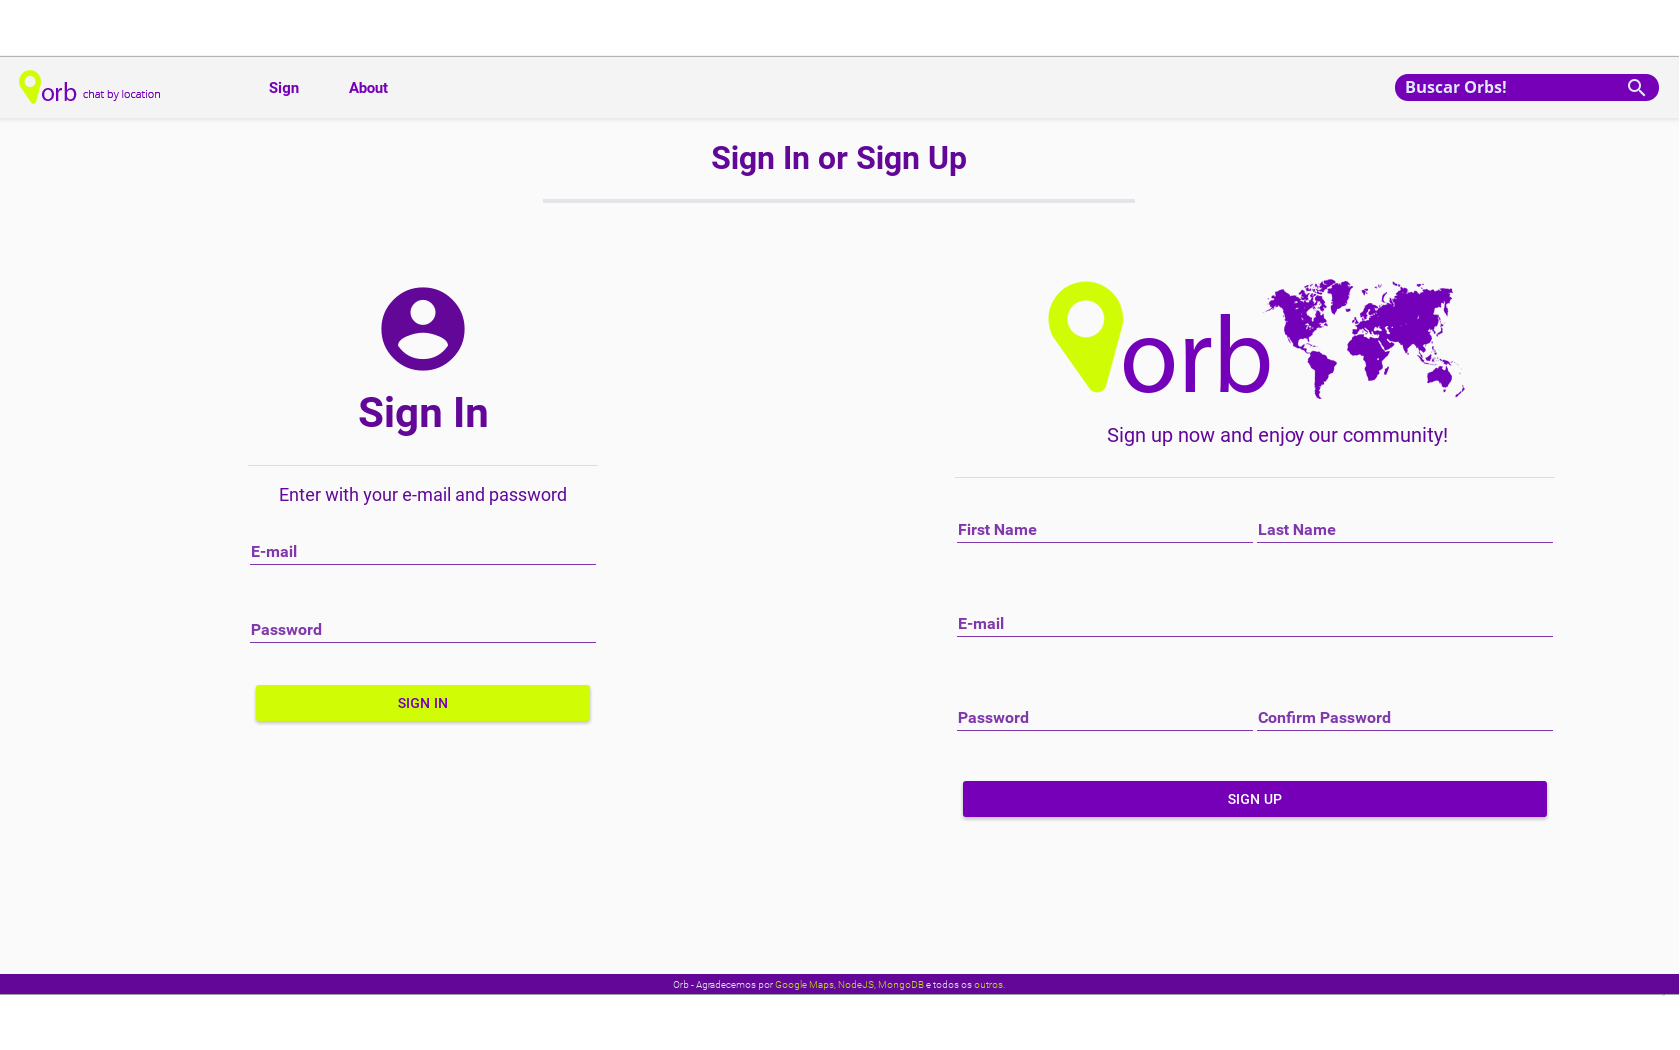
\includegraphics[scale=0.37]{imagens/pagina_signin.png}
	\caption{\small Página de acesso ao sistema.}
	\label{fig:pagina-signin}
\end{figure}

\begin{figure}[!htb]
	\centering
	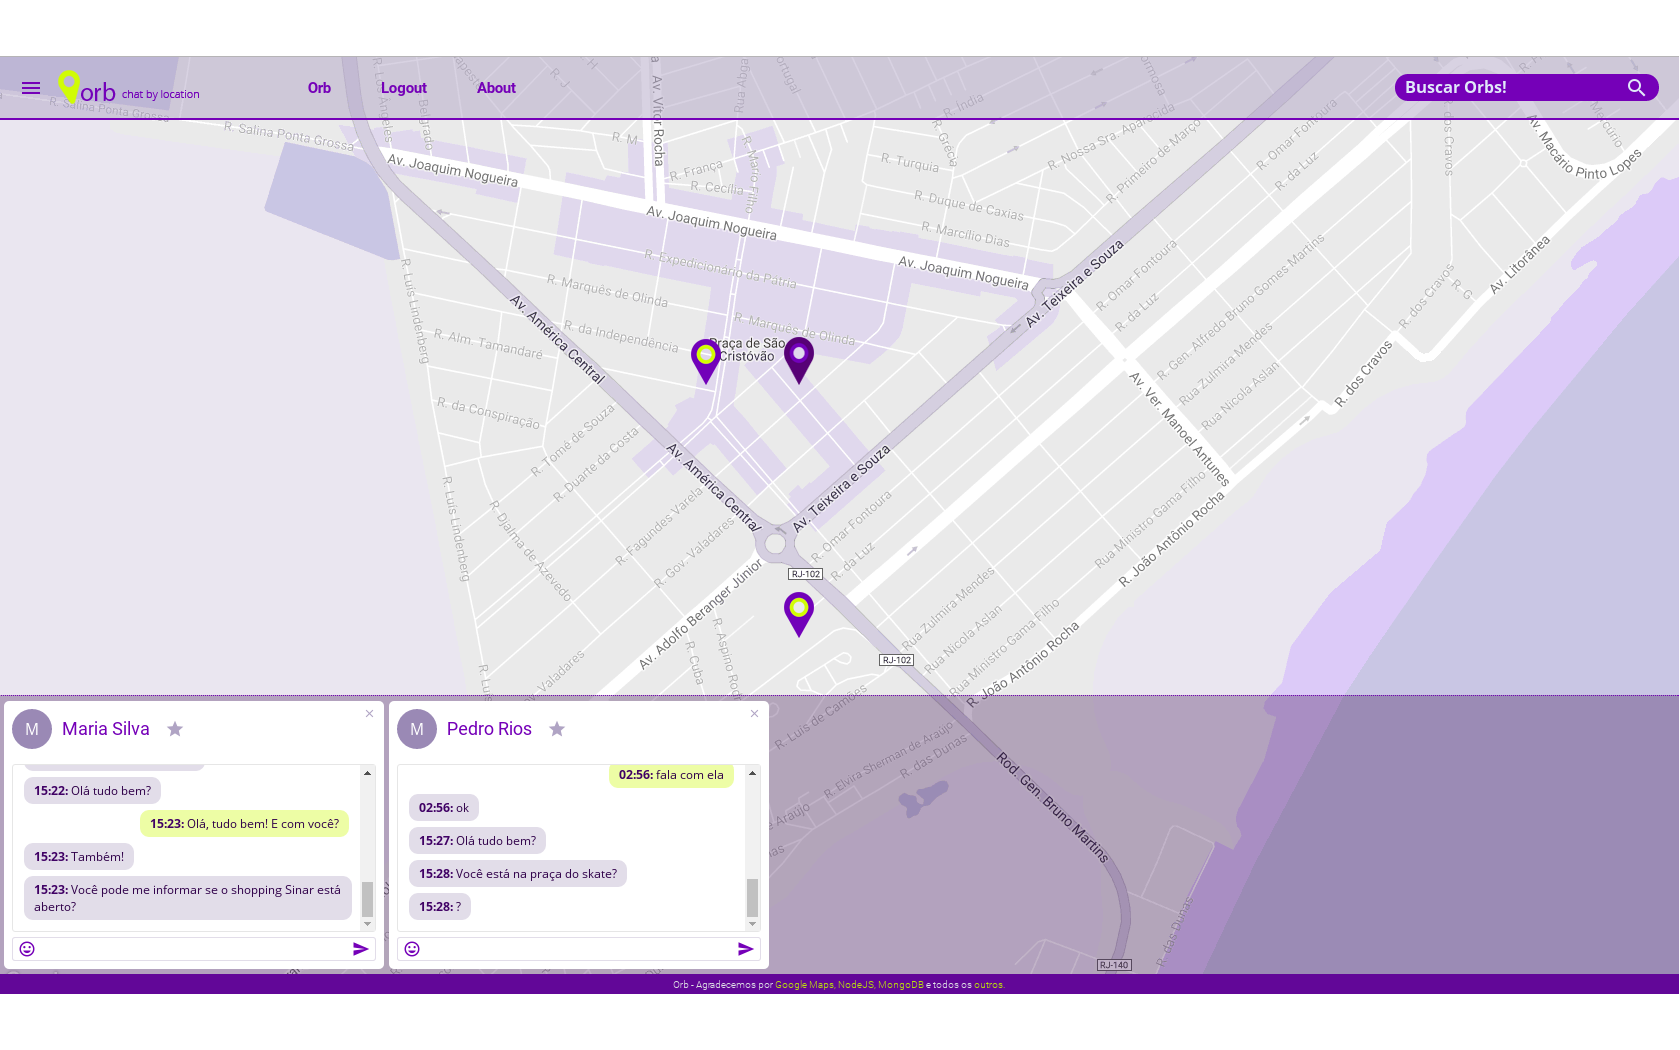
\includegraphics[scale=0.37]{imagens/pagina.png}
	\caption{\small Página principal}
	\label{fig:pagina}
\end{figure}

\begin{figure}[!htb]
	\centering
	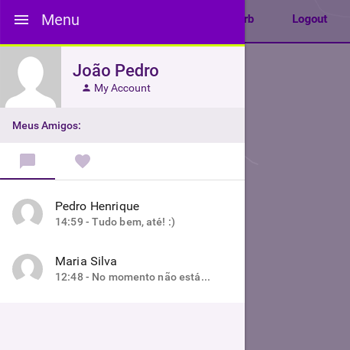
\includegraphics[scale=1]{imagens/aside_menu.png}
	\caption{\small Menu lateral}
	\label{fig:aside-menu}
\end{figure}

\begin{figure}[!htb]
	\centering
	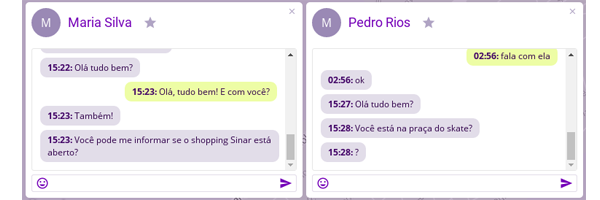
\includegraphics[scale=1]{imagens/chat_panel.png}
	\caption{\small Janelas de \textit{chat}}
	\label{fig:chat-panel}
\end{figure}

	\chapter{Resultados}
	\chapter{Trabalhos Futuros}
A criação das funcionalidades de alterações de informações da conta do usuário e lista de contatos. assim como a validação dos componentes da interface em outros navegadores, como o FireFox, Opera, Safari, Internet Explorer e Microsoft Edge, podem ser implementações rápidas, devido a toda a infraestrutura já estar pronta, assim como a interface, e tornar o sistema útil para algum fim específico que possa se beneficiar das características de comunicação do sistema.

Pensando na utilização por diversos usuários do sistema desenvolvido, existem implementações que devem ser refeitas devido a problemas aparentes de desempenho que a aplicação pode ter, principalmente nas implementações de interação com o mapa, pois a aplicação atual marca todos os usuários \textit{online} no sistema no mapa de cada usuário, o que não é o ideal. Melhorias nesse sentido podem envolver uma pesquisa mais aprofundada nas APIs do Google Maps, para entender melhor as formas de utilização, assim como citamos em trabalhos relacionados, o qual o Uber pode utilizar ferramentas diferentes diferentes para a elaboração do seu mapa. 

Outro ponto importante que envolve este problema de escalabilidade com o sistema de localização, pode ser a utilização das funcionalidades de geolocalização do banco de dados Redis, onde as informações ao invés de serem distribuídas uniformemente para todos os usuários, elas podem ser baseadas na localização do usuário requerente, onde por exemplo, os usuários obtenham informações apenas de outros usuários próximos a ele, fazendo-se cálculos para retorno de dados baseando-se em um determinado raio de distância.

A simulação de ambientes distribuídos e testes de estresse podem ser realizados na aplicação e trazerem resultados interessantes, que podem demonstrar a eficiência da arquitetura desenvolvida para a aplicação. Isto também implicará em novas implementações, como \textit{sticky sessions} e \textit{load balancer}, desmistificando muitos conceitos envolvidos em aplicações que suportam milhares de usuários simultâneos.
	\chapter{Conclusão}
A elaboração deste projeto trabalhou diversas áreas do desenvolvimento de \textit{softwares}, desde a infraestrutura à criação de interfaces. A aplicação de uma tecnologia que proporciona interação em tempo real, foco do nosso tema, foi facilmente introduzida devido as características que as tecnologias escolhidas já propunham, tendo em vista que a \textit{stack} MEAN (MongoDB, ExpressJS, AngularJS, NodeJS) é muito utilizada para a construção de aplicações de tempo real, possibilitando uma pesquisa muito mais fácil devido as diversas soluções semelhantes já elaboradas por outros desenvolvedores.

A exploração deste tema nos proporcionou conhecer algumas das aplicações deste tipo de tecnologia, e principalmente a experiência em se desenvolver uma aplicação deste tipo, tendo em vista a solução que este tipo de tecnologia pode oferecer para diversos problemas tecnológicos. Este trabalho pode contribuir para o entendimento de como utilizar um conjunto de tecnologias para o desenvolvimento de uma aplicação de tempo real, que foi estudado o \textit{chat} como caso de uso. Existem diversas ferramentas de sucesso no mercado que utilizam uma ou mais tecnologias citadas, e demonstram a relevância do tema para o tempo atual da tecnologia, levando a trabalhos cada vez maiores e que exploram as diversas complexidades que sistemas de tempo real podem alcançar para atender as necessidades demandadas. Acreditamos que os resultados alcançados atingiram as metas propostas pelo trabalho, e deixam abertas oportunidades para pesquisas mais específicas da tecnologia.

A ideia deste trabalho também foi ser como um passo inicial para o entendimento do ambiente de tempo real em aplicações, consequentemente não aplicamos e nem nos aprofundamos em algumas boas práticas, como o desenvolvimento orientado a testes, o que tornou a utilidade da aplicação meramente demonstrativa, mas que com mais trabalho pode se tornar algo utilizável para outros futuros estudos na área em que abrange.

\section{Trabalhos Futuros}
Para trabalhos futuros a criação das funcionalidades de alterações de informações da conta do usuário e lista de contatos. assim como a validação dos componentes da interface em outros navegadores, como o FireFox, Opera, Safari, Internet Explorer e Microsoft Edge, podem ser implementações rápidas, devido a toda a infraestrutura já estar pronta, assim como a interface, e tornar o sistema útil para algum fim específico que possa se beneficiar das características de comunicação do sistema.

Pensando na utilização por diversos usuários do sistema desenvolvido, existem implementações que devem ser refeitas devido a problemas aparentes de desempenho que a aplicação pode ter, principalmente nas implementações de interação com o mapa, pois a aplicação atual marca todos os usuários \textit{online} no sistema no mapa de cada usuário, o que não é o ideal, pois no caso de muitos usuários online, a marcação de muitos pontos no mapa poderá causar lentidão ou até paralisação total da página. Melhorias nesse sentido podem envolver uma pesquisa mais aprofundada nas APIs do Google Maps, para entender melhor as formas de utilização, assim como citamos em trabalhos relacionados, o qual o Uber pode utilizar ferramentas diferentes diferentes para a elaboração do seu mapa. 

Outro ponto importante que envolve este problema de escalabilidade com o sistema de localização, pode ser a utilização das funcionalidades de geolocalização do banco de dados Redis, onde as informações ao invés de serem distribuídas uniformemente para todos os usuários, elas podem ser baseadas na localização do usuário requerente, onde por exemplo, os usuários obtenham informações apenas de outros usuários próximos a ele, fazendo-se cálculos para retorno de dados baseando-se em um determinado raio de distância.

A simulação de ambientes distribuídos e testes de estresse podem ser realizados na aplicação para demonstrar a eficiência da arquitetura desenvolvida para a aplicação. Isto também implicará em novas implementações, como \textit{sticky sessions} e \textit{load balancer}, mostrando muitos conceitos envolvidos em aplicações que suportam milhares de usuários simultâneos.

	
	%===================================================================================
	%\backmatter
	%===================================================================================
	
	%\bibliography{monografia}{}
	%\bibliographystyle{abnt-alf}
	
	% OUTRA FORMA DE CRIAR A BIBLIOGRAFIA:
	\begin{thebibliography}{9}
		\bibitem{startup-email-innovation1}Liveclicker Delivers Dynamic Messaging Capability with RealTime Email Solution. Disponível em: \url{http://www.destinationcrm.com/Articles/CRM-News/CRM-Featured-News/Liveclicker-Delivers-Dynamic-Messaging-Capability-with-RealTime-Email-Solution-97439.aspx}.
		Acesso em: 19 Out. 2016.
		
		\bibitem{startup-email-innovation2}Liveclicker RealTime Email Solution. Disponível em: \url{http://www.realtime.email/}.
		Acesso em: 19 Out. 2016.
		
		\bibitem{uber-statistics}50 Amazing Uber Statistics (October 2016). Disponível em: \url{http://expandedramblings.com/index.php/uber-statistics/}.
		Acesso em: 20 Out. 2016.
		
		\bibitem{uber}Uber. Disponível em: \url{https://www.uber.com/}.
		Acesso em: 20 Out. 2016.
		
		\bibitem{uber-how-scales}How Uber Scales Their Real-Time Market Platform. Disponível em: \url{http://highscalability.com/blog/2015/9/14/how-uber-scales-their-real-time-market-platform.html}.
		Acesso em: 20 Out. 2016.
		
		\bibitem{redis-pubsub-redismva}Redis Publish-Subscribe (RedisMVA). Disponível em: \url{https://github.com/sayar/RedisMVA/blob/master/module6_redis_pubsub/README.md#redis-publish-subscribe}.
		Acesso em: 20 Out. 2016.
		
		\bibitem{browsers-usage}Web browsers usage table. Disponível em: \url{http://caniuse.com/usage-table}.
		Acesso em: 20 Out. 2016.
		
		\bibitem{redis-pubsub-rajaraodv}Redis Pub/Sub (Rajaraodv). Disponível em: \url{https://github.com/rajaraodv/redispubsub}.
		Acesso em: 20 Out. 2016.
		
		\bibitem{fanmappr}FanMappr. Disponível em: \url{http://h.fanapp.mobi/modules/fanmappr/fanmappr.php?fid=1056666}.
		Acesso em: 20 Out. 2016.
		
		\bibitem{radiusim}RadiusIM – Social Messenger Com Busca Por Geotagging. Disponível em: \url{http://br.wwwhatsnew.com/2008/09/radiusim-%E2%80%93-social-messenger-por-com-busca-por-geotagging/}.
			Acesso em: 20 Out. 2016.
			
		\bibitem{notnotcitricsquid}NOTNOTCITRICSQUID. Do location based chat apps start trending again?. Disponível em: \url{https://www.reddit.com/r/startups/comments/1tkc3f/do_location_based_chat_apps_start_trending_again/}.
		Acesso em: 21 Out. 2016.
		
		\bibitem{snapchat}Snapchat. Disponível em: \url{https://www.snapchat.com/}.
		Acesso em: 21 Out. 2016.
		
		\bibitem{tinder}Tinder. Disponível em: \url{https://www.gotinder.com/}.
		Acesso em: 21 Out. 2016.
		
		\bibitem{happn}Happn. Disponível em: \url{https://www.happn.com/}.
		Acesso em: 21 Out. 2016.
		
		\bibitem{internet-traffic-stats1}How Much Web Traffic Is On Mobile Devices (Really)? Disponível em: \url{https://keriganmarketing.com/freelunch/view/how-much-web-traffic-is-on-mobile-devices/}.
		Acesso em: 22 Out. 2016.
		
		\bibitem{internet-traffic-stats2}Internet stats and facts for 2016. Disponível em: \url{https://hostingfacts.com/internet-facts-stats-2016/}.
		Acesso em: 22 Out. 2016.
		
		\bibitem{internet-traffic-stats3}Mobile Marketing Statistics compilation. Disponível em: \url{http://www.smartinsights.com/mobile-marketing/mobile-marketing-analytics/mobile-marketing-statistics/}.
		Acesso em: 22 Out. 2016.
		
		\bibitem{notebook-info}Notebook HP 1000-1460BR. Disponível em: \url{http://www.lojahp.com.br/Voce/Notebook/Notebook-HP-1000-1460BR-com-Intel-Core-i5-3230M-Windows-8-4GB-500GB-Gravador-de-DVD-Leitor-de-Cartoes-HDMI-e-LED-14-2177574.html}.
		Acesso em: 24 Out. 2016.
		
		\bibitem{facebook-distro}Facebook Linux, What Distro is it?. Disponível em: \url{http://www.internetnews.com/blog/skerner/facebook-linux-CentOS.html}.
		Acesso em: 24 Out. 2016.
		
		\bibitem{google-redhat}Red Hat Enterprise Linux Atomic Host expands to Google Compute Engine. Disponível em: \url{https://cloudplatform.googleblog.com/2014/07/red-hat-enterprise-linux-atomic-host-expands-to-google-compute-engine.html?m=1}.
		Acesso em: 24 Out. 2016.
		
		\bibitem{gitflow}Gitflow Workflow. Disponível em: \url{https://www.atlassian.com/git/tutorials/comparing-workflows/gitflow-workflow}.
		Acesso em: 24 Out. 2016.
		
		\bibitem{sublime}Sublime Text. Disponível em: \url{https://www.sublimetext.com/}.
		Acesso em: 24 Out. 2016.
		
		\bibitem{packagecontrolio}Package Control. Disponível em: \url{https://packagecontrol.io/}.
		Acesso em: 24 Out. 2016.
		
		\bibitem{vscode}Visual Studio Code. Disponível em: \url{https://code.visualstudio.com/}.
		Acesso em: 24 Out. 2016.
		
		\bibitem{nodejs}NodeJS. Disponível em: \url{https://nodejs.org/}.
		Acesso em: 24 Out. 2016.
		
		\bibitem{v8}Chrome V8. Disponível em: \url{https://developers.google.com/v8/}.
		Acesso em: 24 Out. 2016.
		
		\bibitem{img-eventloop}Introdução ao Node.js. Disponível em: \url{http://maxroecker.github.io/blog/introducao-ao-nodejs/}.
		Acesso em: 24 Out. 2016.
		
		\bibitem{libuv}Libuv. Disponível em: \url{https://github.com/libuv/libuv}.
		Acesso em: 24 Out. 2016.
		
		\bibitem{npm}NPM. Disponível em: \url{https://www.npmjs.com/}.
		Acesso em: 24 Out. 2016.
		
		\bibitem{expressjs}ExpressJS. Disponível em: \url{https://expressjs.com/}.
		Acesso em: 24 Out. 2016.
		
	\end{thebibliography}
		\anexo
	\end{document}